%
% Chapter 9
%

\chapter{SIGNAL EXTRACTION}
Despite the event selection being aimed at selecting signal and rejecting background, the signal region yields are dominated by background events,
and lack sufficient statistics to identify the presence of the \tth signal in data. These post-selection (pre-fit) yields are in Table~\ref{tab:yields} below.
Becuse the post-selection yields offer no discernable way of separating the signal in the data, additional discrimination is necessary. A multivariate strategy
relying on Boosted Decision Trees (BDTs) is used to further discriminate the \tth signal from various backgrounds. 

\begin{table}[htbp]
\begin{center}
  \caption[Signal region event yields by lepton flavor]{Expected (pre-fit) yields for signal and background processes, and observed yields in data. Uncertainties shown
are purely statistical.}
    \begin{tabular}{l c c c} \hline
& $\mu\mu$ & $ee$ & $e\mu$  \\ \hline 
$t\bar{t}W$ & 45.4 $\pm$ 0.5 & 17.8 $\pm$ 0.3 & 64.3 $\pm$ 0.6 \\
$t\bar{t}Z/\gamma^{*}$ & 16.8 $\pm$ 0.7 & 14.8 $\pm$ 0.8 & 41.7 $\pm$ 1.4 \\
\hline
WZ & 5.2 $\pm$ 0.7 & 1.6 $\pm$ 0.4 & 7.5 $\pm$ 0.8 \\
Rare SM. bkg & 6.8 $\pm$ 0.3 & 3.5 $\pm$ 0.2 & 11.7 $\pm$ 0.4 \\
WWss & 2.9 $\pm$ 0.2 & 1.4 $\pm$ 0.1 & 4.3 $\pm$ 0.2 \\
\hline
Conversions & 0.0 $\pm$ 0.0 & 3.4 $\pm$ 1.1 & 8.5 $\pm$ 1.3 \\
Charge flip & 0.0 $\pm$ 0.0 & 172 $\pm$ 93 & 149 $\pm$ 82 \\
Non-prompt leptons & 29.9 $\pm$ 1.2 & 17.3 $\pm$ 1.1 & 53.5 $\pm$ 1.8 \\
\hline
Total bkg & 107.3 $\pm$ 1.7 & 70.3 $\pm$ 1.8 & 208.0 $\pm$ 2.9 \\
 \hline
$t\bar{t}H$ & 18.5 $\pm$ 0.2 & 7.4 $\pm$ 0.1 & 26.2 $\pm$ 0.2 \\
 \hline
Data & 154 & 95 & 274 \\
\hline
\end{tabular}
    \label{tab:yields}
\end{center}
\end{table}

The signal extraction strategy adopted here targets the two largest backgrounds, \ttv and the non-prompt leptons, and uses BDTs to discriminate against each separately.
The inputs to these BDTs include event kinematics, as well as outputs of other BDTs, designed to resconstruct parts of the signal events such as the Higgs jets and the
hadronically decaying top quark. Finally, the outputs of the BDT dscriminators are binned in a uniqe approach which produces a final shape template that is used
for the final results.

\section{Two Dimensional BDTs}
\label{sec:2D_BDT}
Two BDTs are used to produce the final shape template. One BDT is trained exclusively against the \ttv background, while the other targets the background due to non-prompt
leptons. Because the non-prompt background is a data-driven estimation, all of the events making up this background cannot be used for MVA training, since the BDT must be
trained on a completely separate set of events from the set it is evaluated on. Because a large part of the fake background is comprised of the \ttbar process, the BDT is
trained against \ttbar MC. The outputs of the two BDTs are plotted on separate axes forming a two-dimensional shape. This two-dimensional shape is binned into rectangles
and the contents of which form a one-dimensional histogram. 

A loosened version of the $2lss$ signal region selection is applied to the training events. This loosened selection is motivated by increasing the training statistics available
while not affecting the behavior and kinematics of the input variables with respect to the signal region. This loosened selection consists of the following criteria:
\begin{itemize}
\item At least two preselected same-sign leptons
\item The lepton \pt $>$ 25,15 
\item At least 4 preselected jets among which there must be $\geq$ 2 CSVv2 L or $\geq$ 1 CSVv2 M
\end{itemize}

The input variables are selected considering not only the best individual separation power, but also the set that offers the best discrimination power of the BDT. These two
properties are not necessarily the same, since correlations and anti-correlations among varibles can differ substantially between signal and background, providing significant
discrimination power. Additionally, the closure between MC and data, also known as modeling, was considered since variables that are not modeled well in MC cannot be used to
approximate the variable's behavior in data. The input variables used for the BDT training against \ttbar include:
\begin{itemize}
\item the absolute value of the maximum psuedorapidity of the two leptons
\item the multiplicity of hadronic jets
\item the minimum angular distance between the leading lepton and the nearest jet
\item the minimum angular distance between the trailing lepton and the nearest jet
\item the transverse mass of the leading lepton and missing transverse energy
\item the hadronic top reconstruction score
\end{itemize} 

\noindent the input variables used for the BDT training against \ttv include:
\begin{itemize}
\item the absolute value of the maximum psuedorapidity of the two leptons
\item the multiplicity of hadronic jets
\item the minimum angular distance between the leading lepton and the nearest jet
\item the minimum angular distance between the trailing lepton and the nearest jet
\item the transverse mass of the leading lepton and missing transverse energy
\item the leading lepton transverse momentum
\item the trailing lepton transverse momentum
\item the Higgs jet tagger score after hadronic top removal
\end{itemize} 

\noindent The discrimination power of these input variables against the largest backgrounds is available in Figures~\ref{fig:inputs1}~\ref{fig:inputs2}~\ref{fig:inputs3}.
The reconstruction inputs offer improved discrimination power against both of the largest backgrounds, see Figure~\ref{fig:inputs3}.

\begin{figure}[htp]
\centering
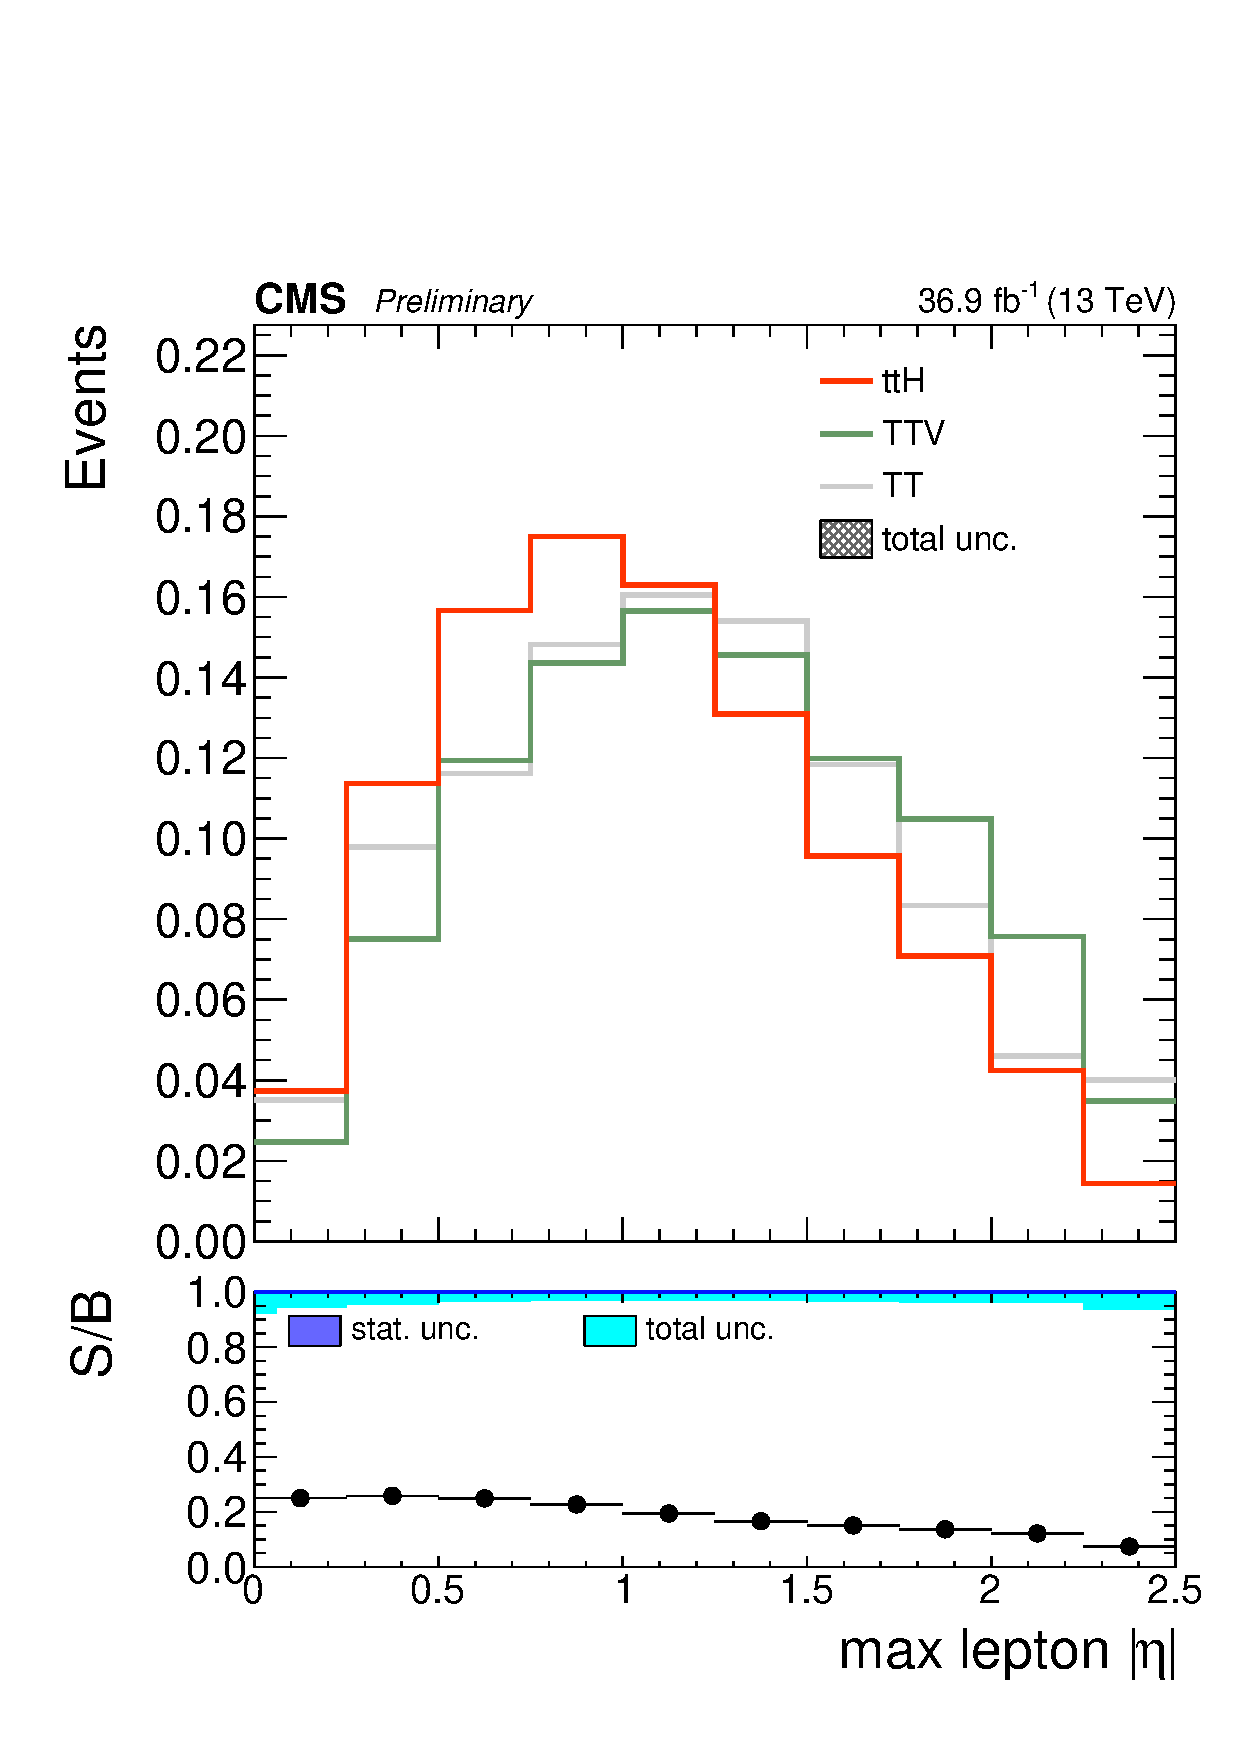
\includegraphics[width=0.3\textwidth]{ch9_figs/kinMVA_input_max_Lep_eta.pdf}
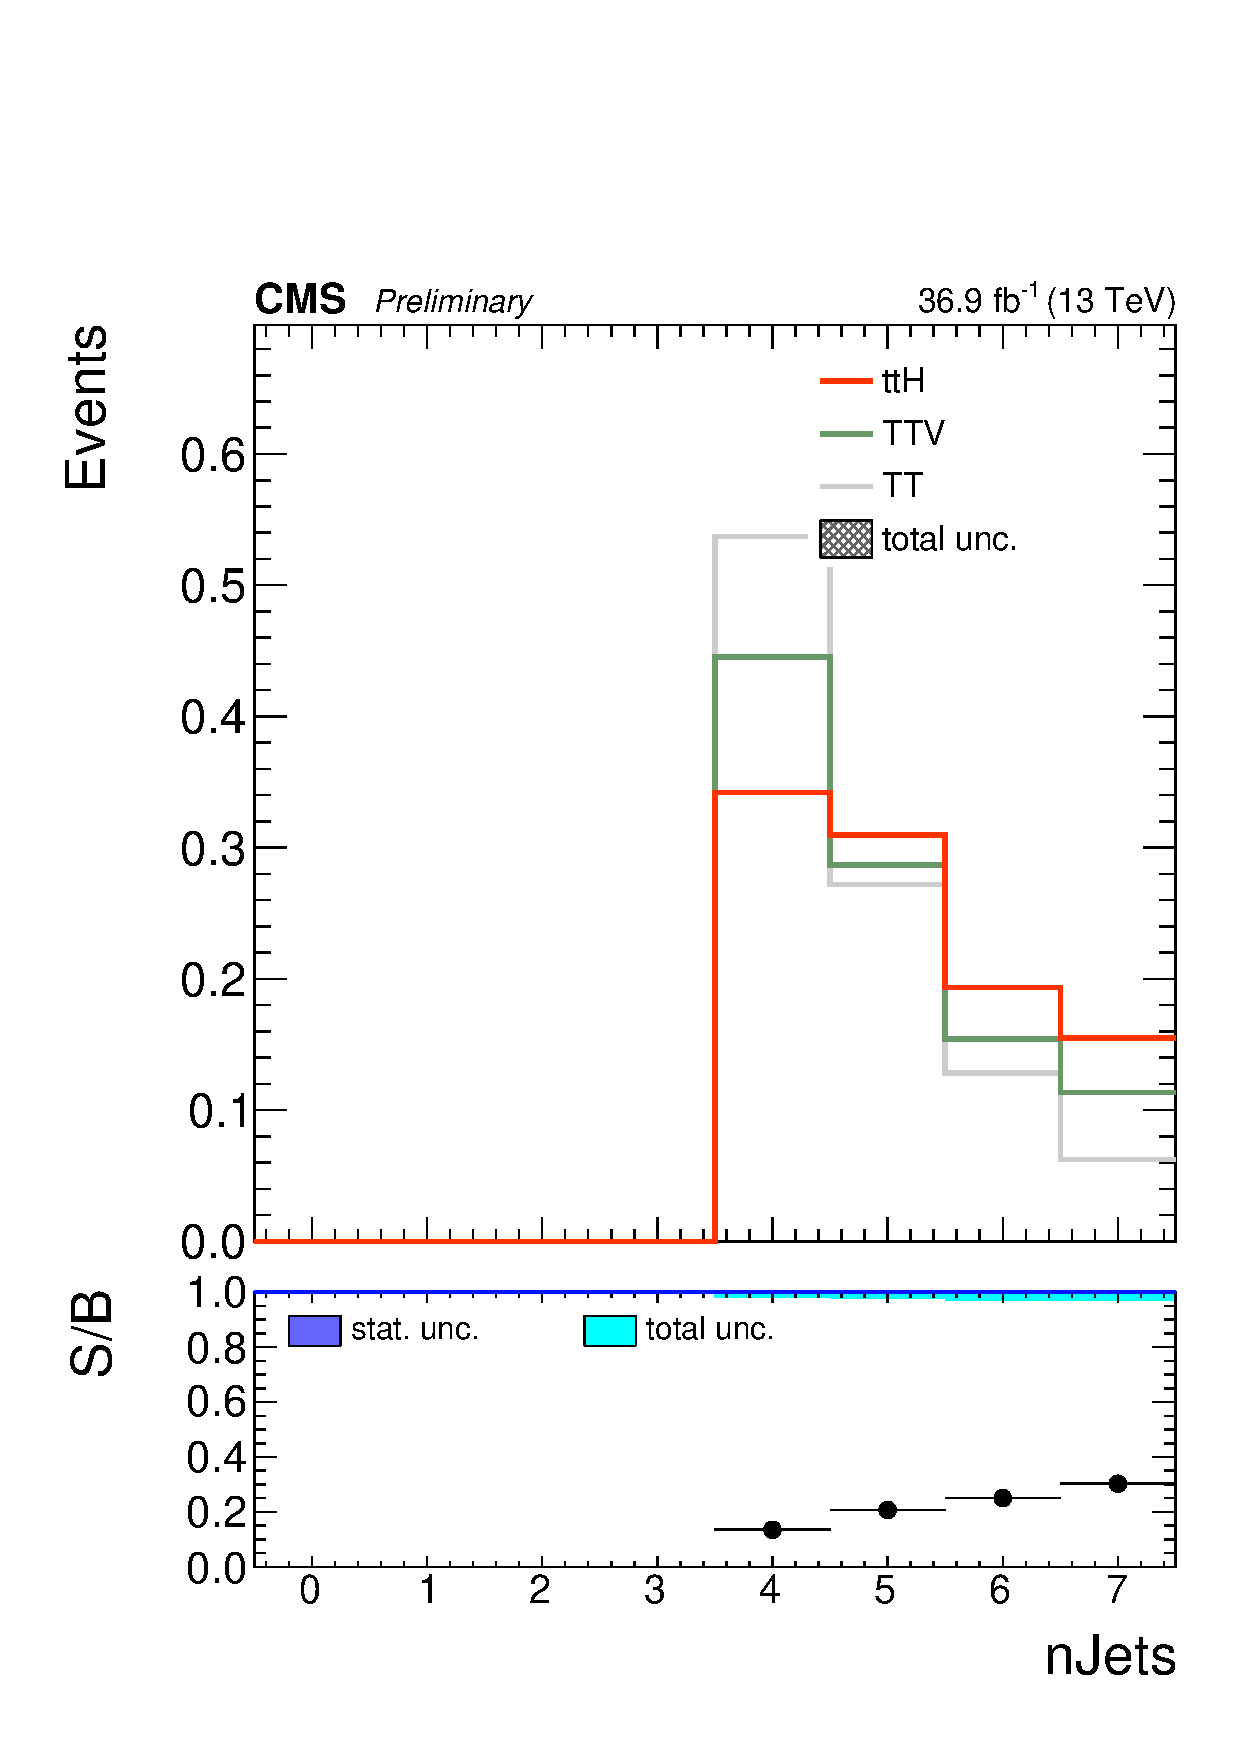
\includegraphics[width=0.3\textwidth]{ch9_figs/kinMVA_input_numJets.pdf}
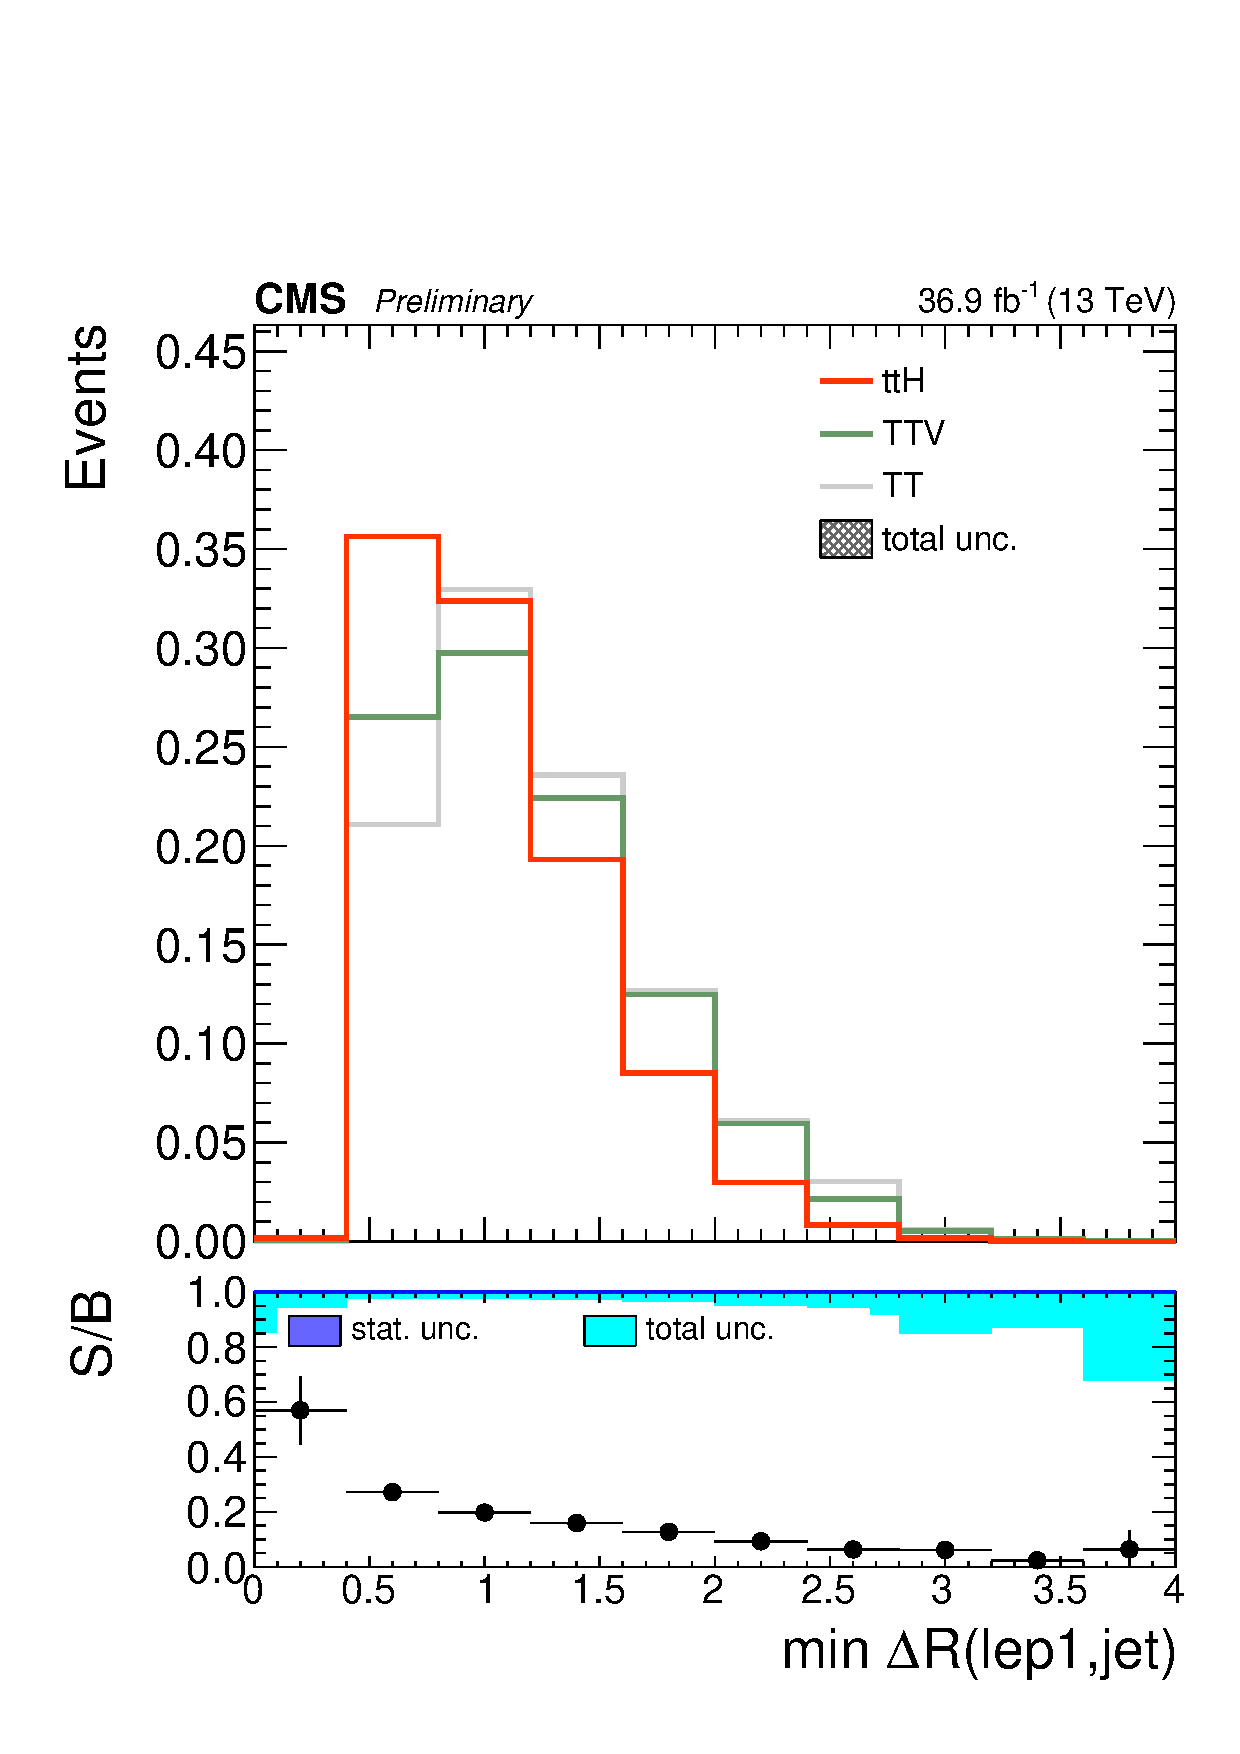
\includegraphics[width=0.3\textwidth]{ch9_figs/kinMVA_input_mindr_lep1_jet.pdf}

\caption[Signal extraction BDT input variables]{Separtion power among various backgrounds for BDT input variables}
\label{fig:inputs1}
\end{figure}

\begin{figure}[htp]
\centering
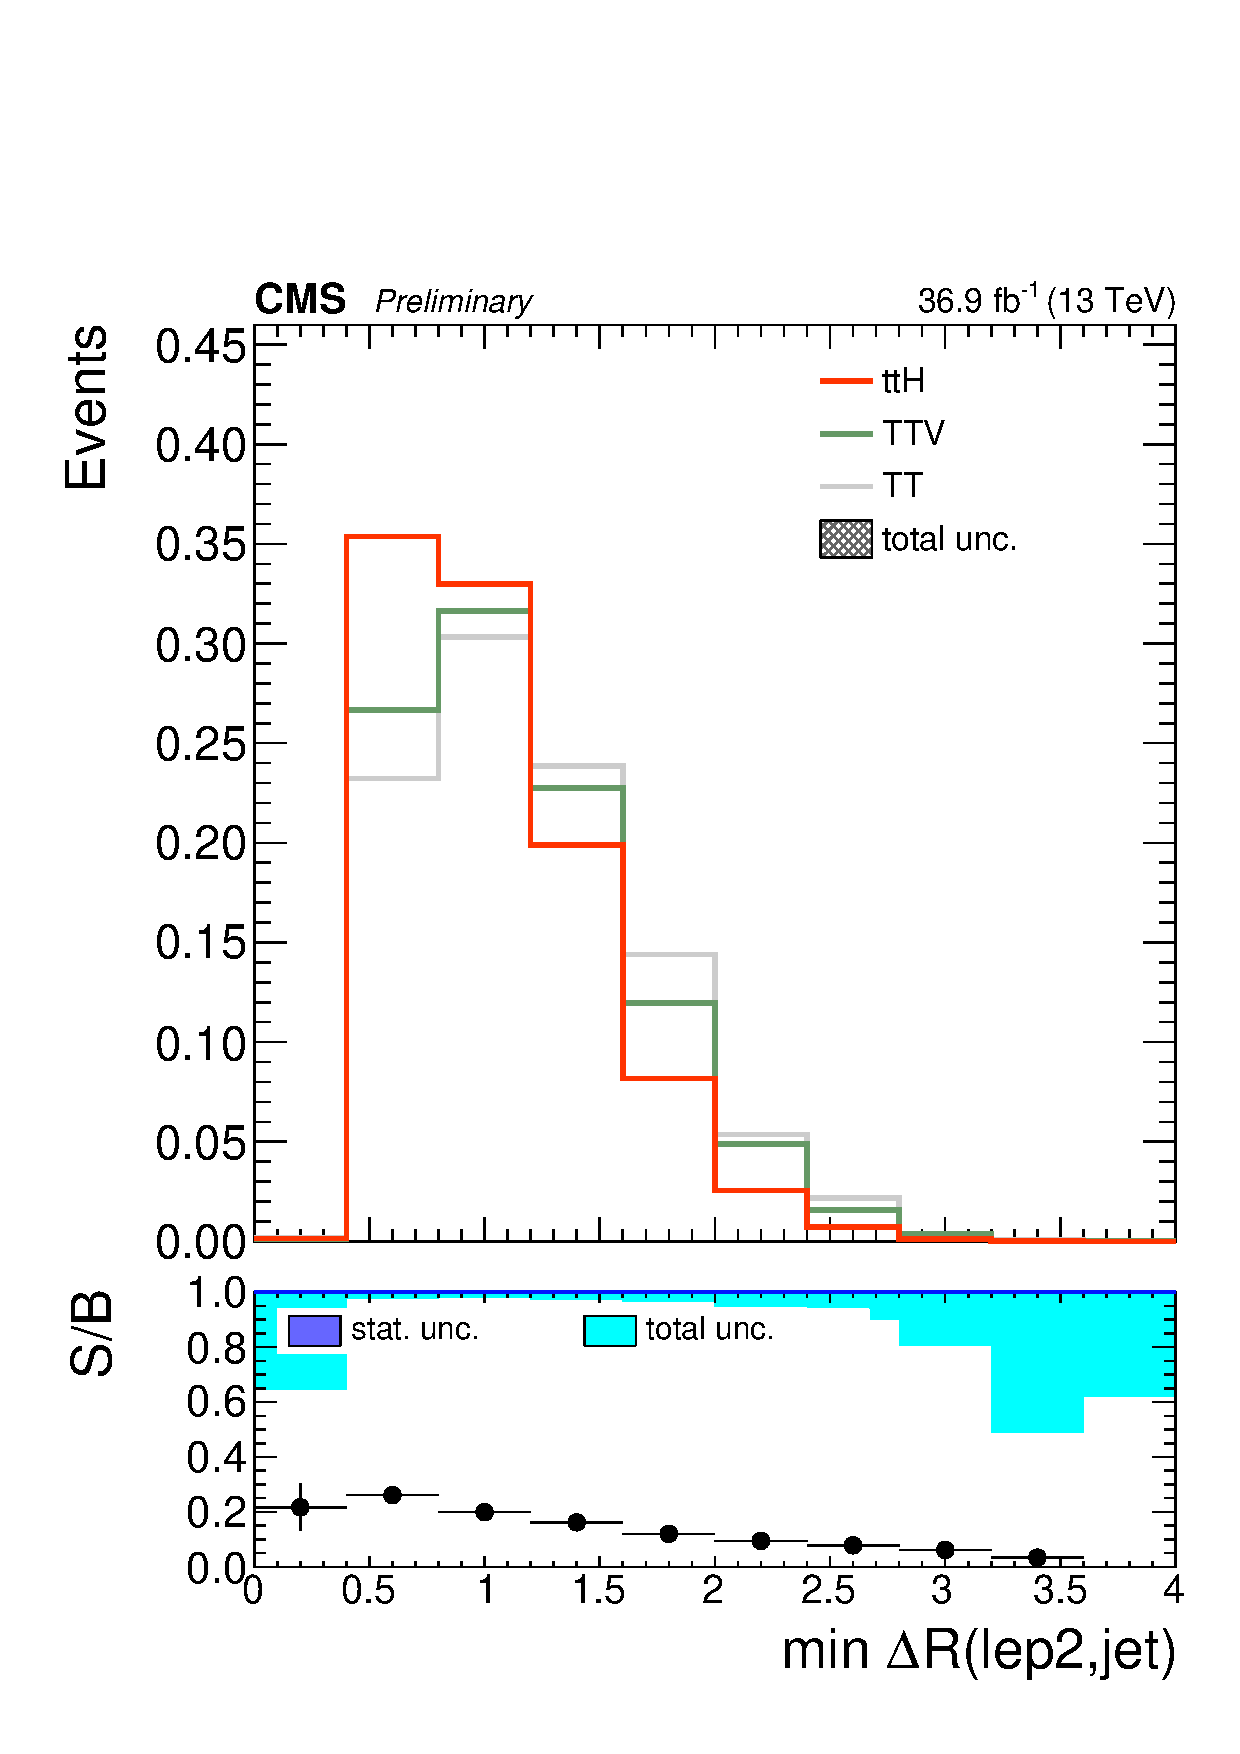
\includegraphics[width=0.3\textwidth]{ch9_figs/kinMVA_input_mindr_lep2_jet.pdf}
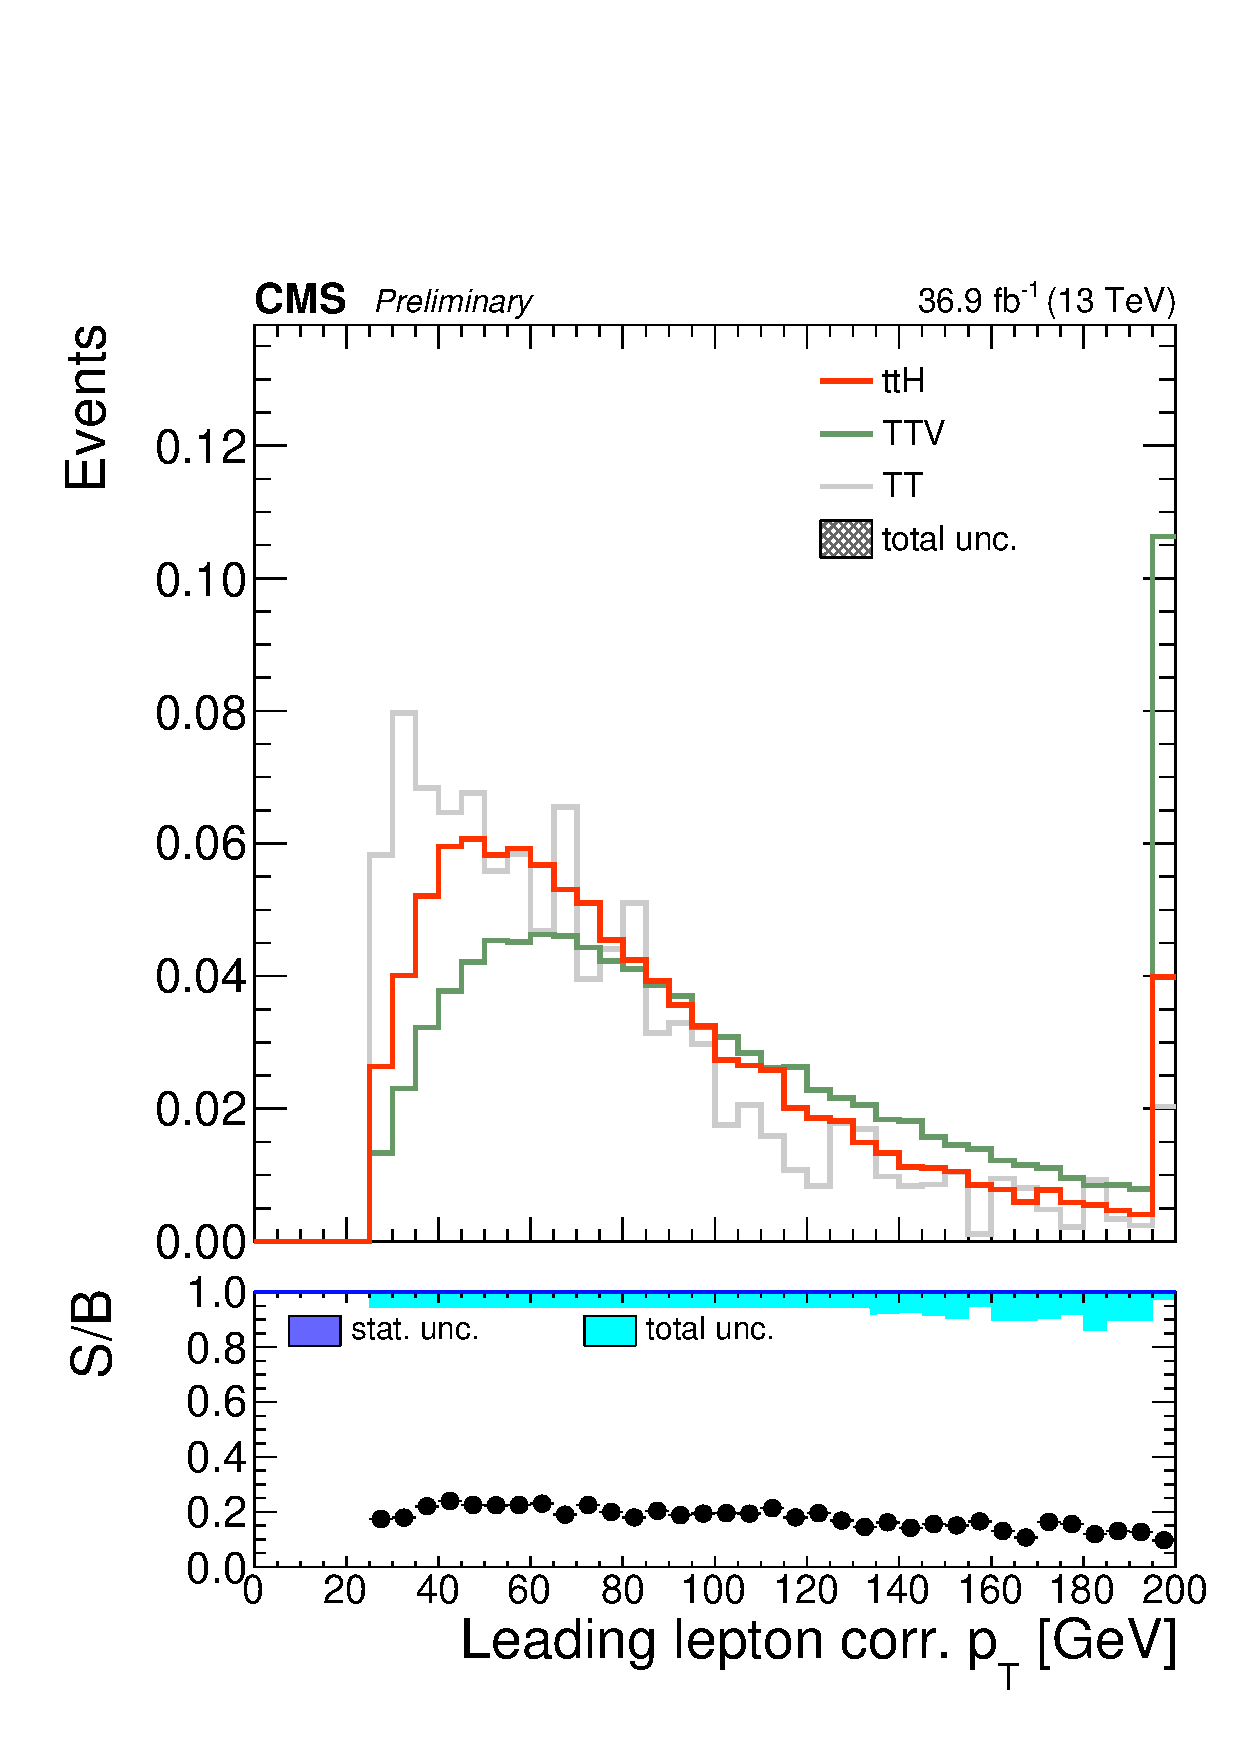
\includegraphics[width=0.3\textwidth]{ch9_figs/kinMVA_input_LepGood0_conePt.pdf}
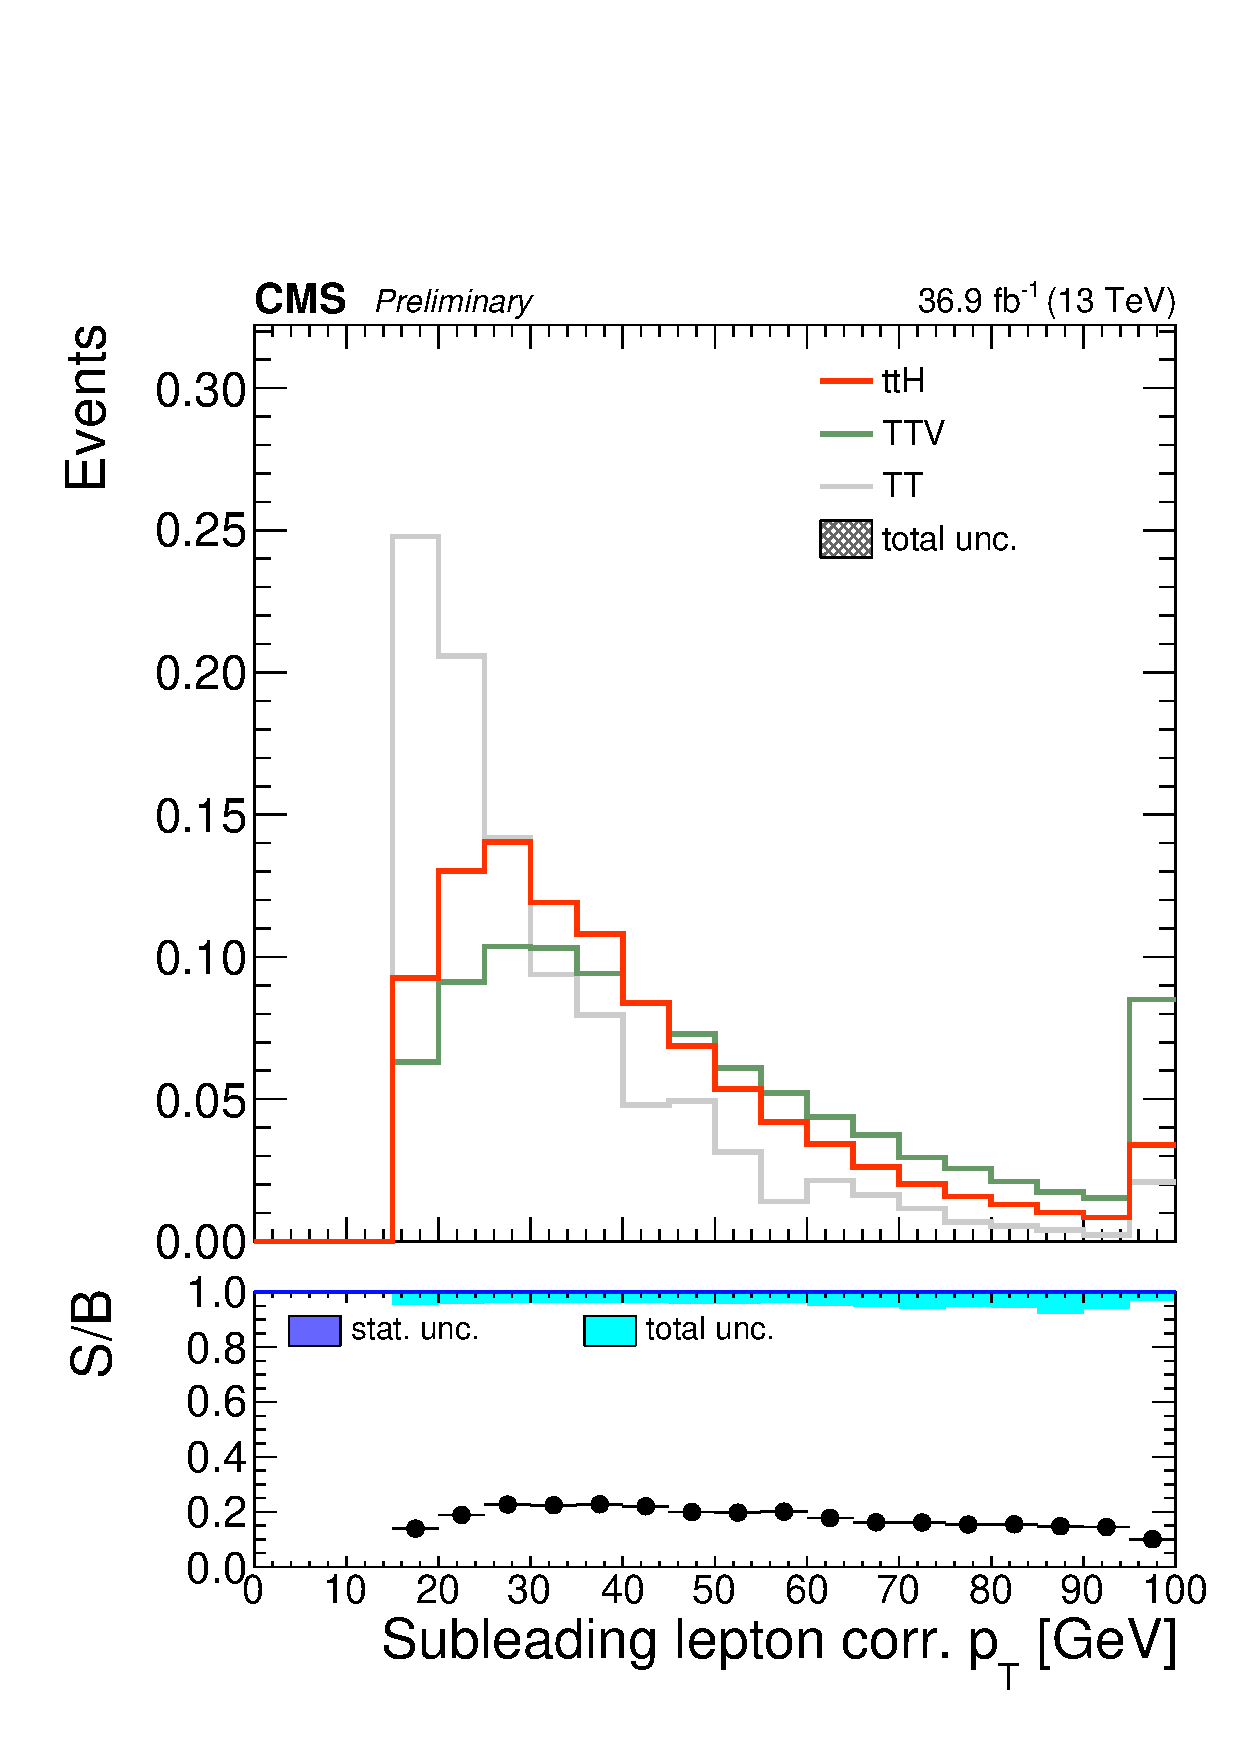
\includegraphics[width=0.3\textwidth]{ch9_figs/kinMVA_input_LepGood1_conePt.pdf}
\caption[Signal extraction BDT input variables]{Separtion power among various backgrounds for BDT input variables}
\label{fig:inputs2}
\end{figure}

\begin{figure}[htp]
\centering
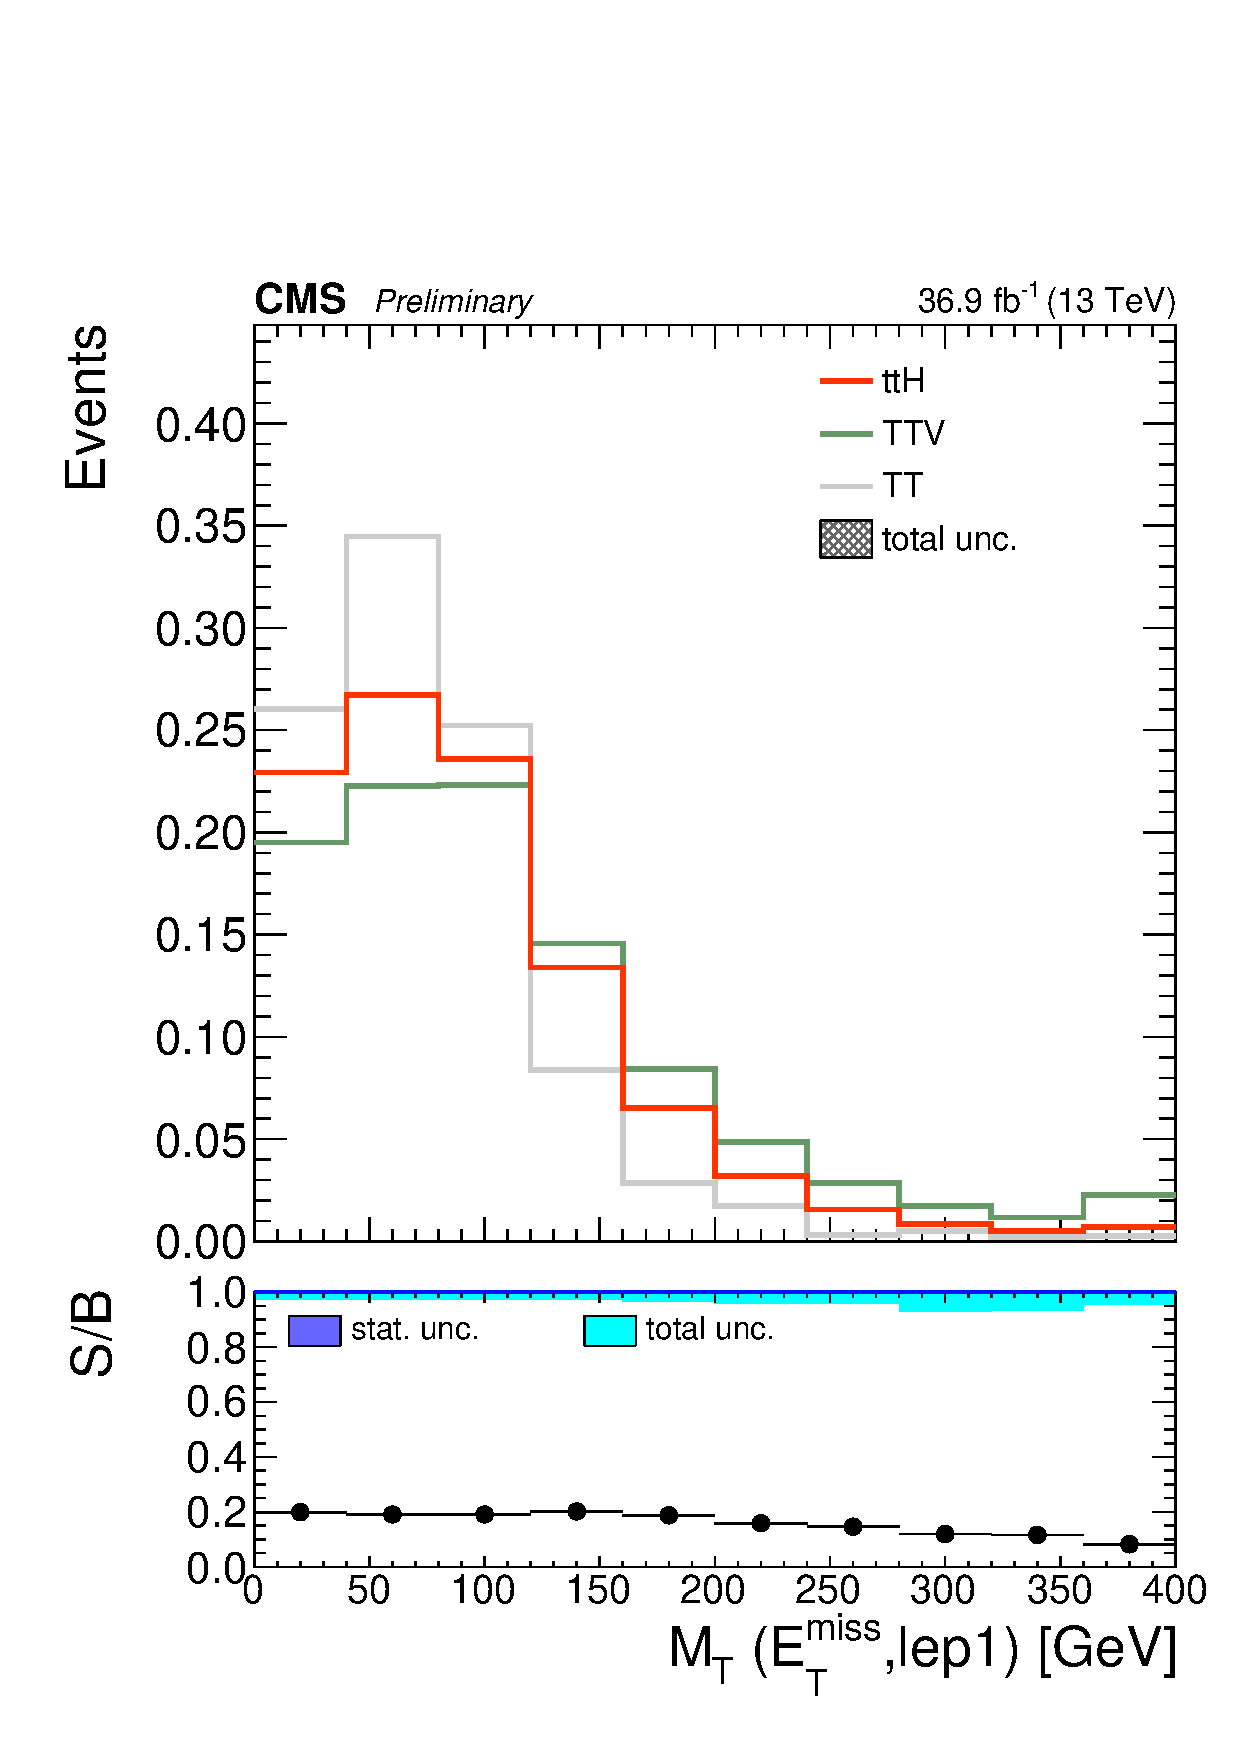
\includegraphics[width=0.3\textwidth]{ch9_figs/kinMVA_input_MT_met_lep1.pdf}
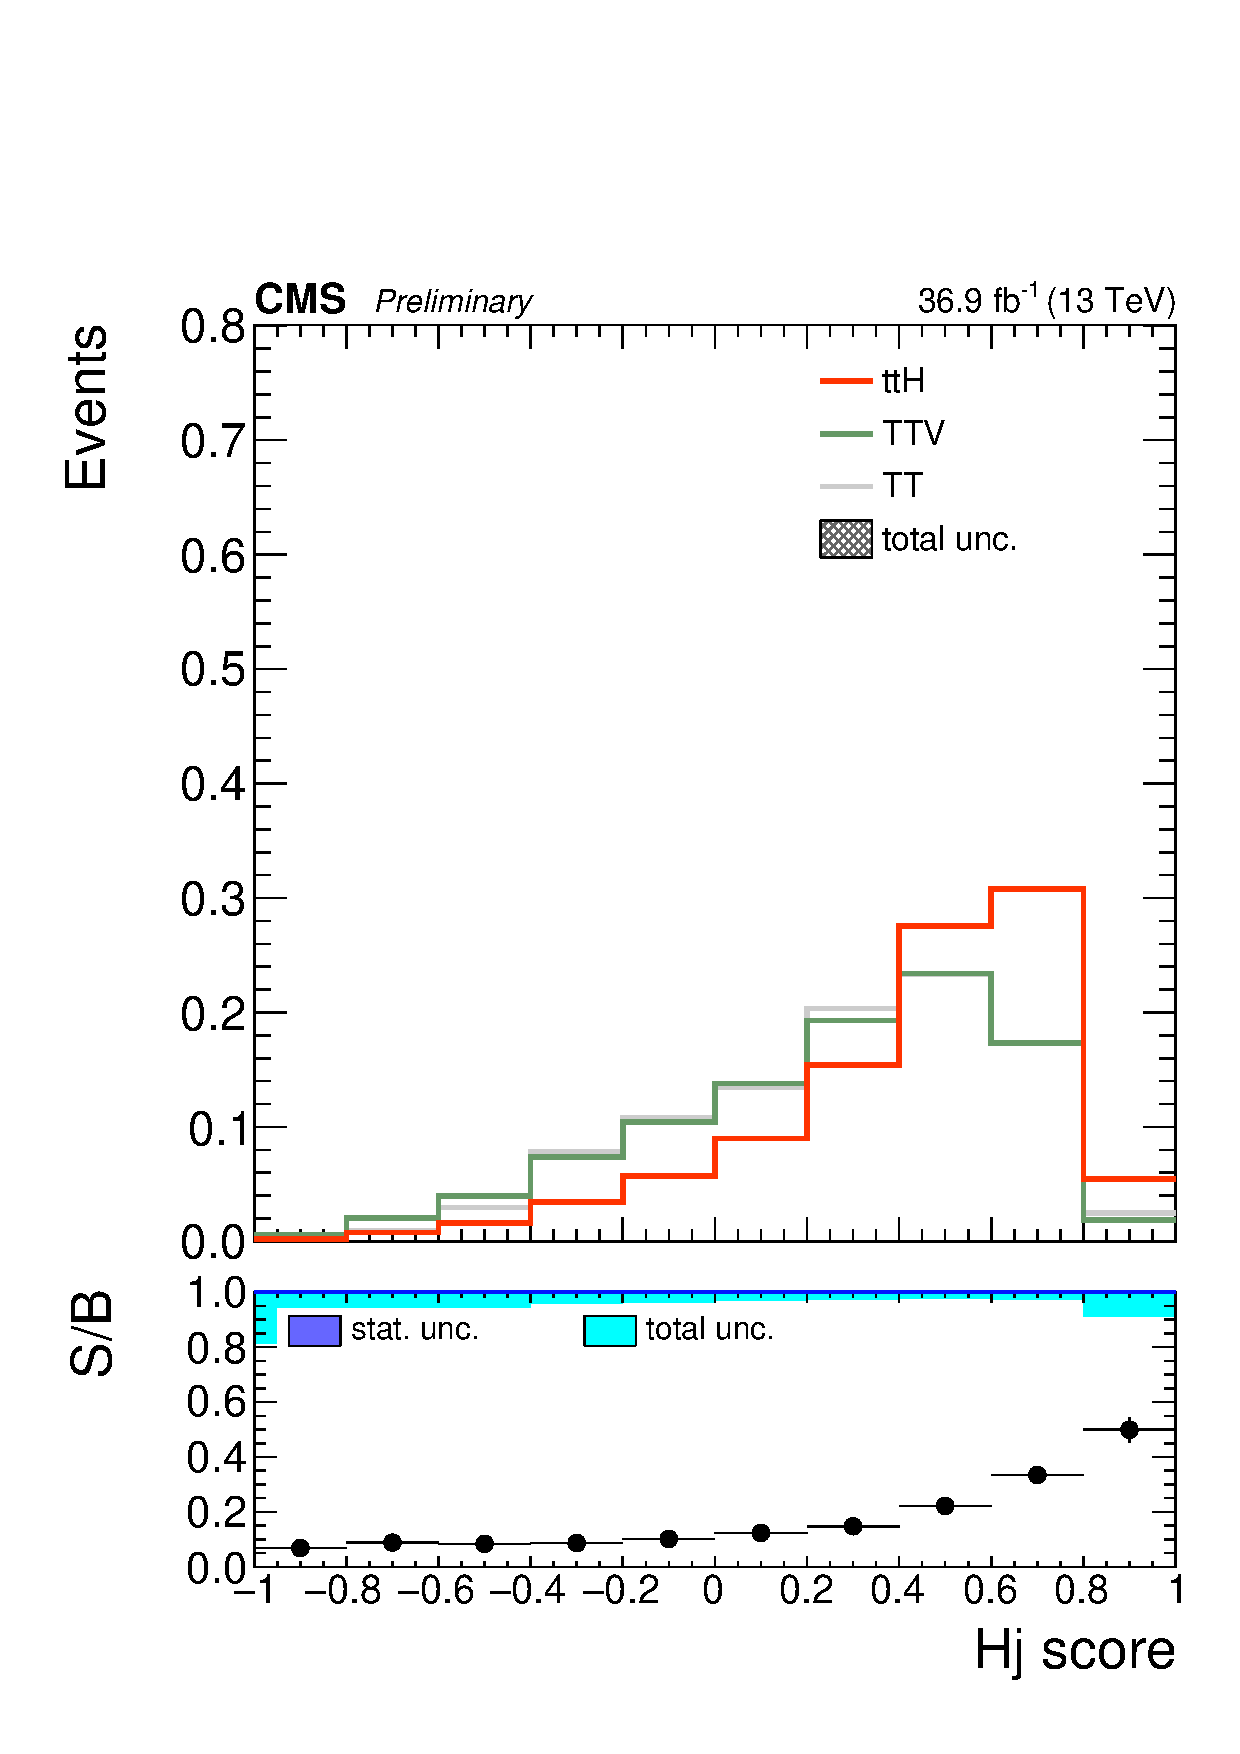
\includegraphics[width=0.3\textwidth]{ch9_figs/kinMVA_input_BDTv8_eventReco_Hj_score.pdf}
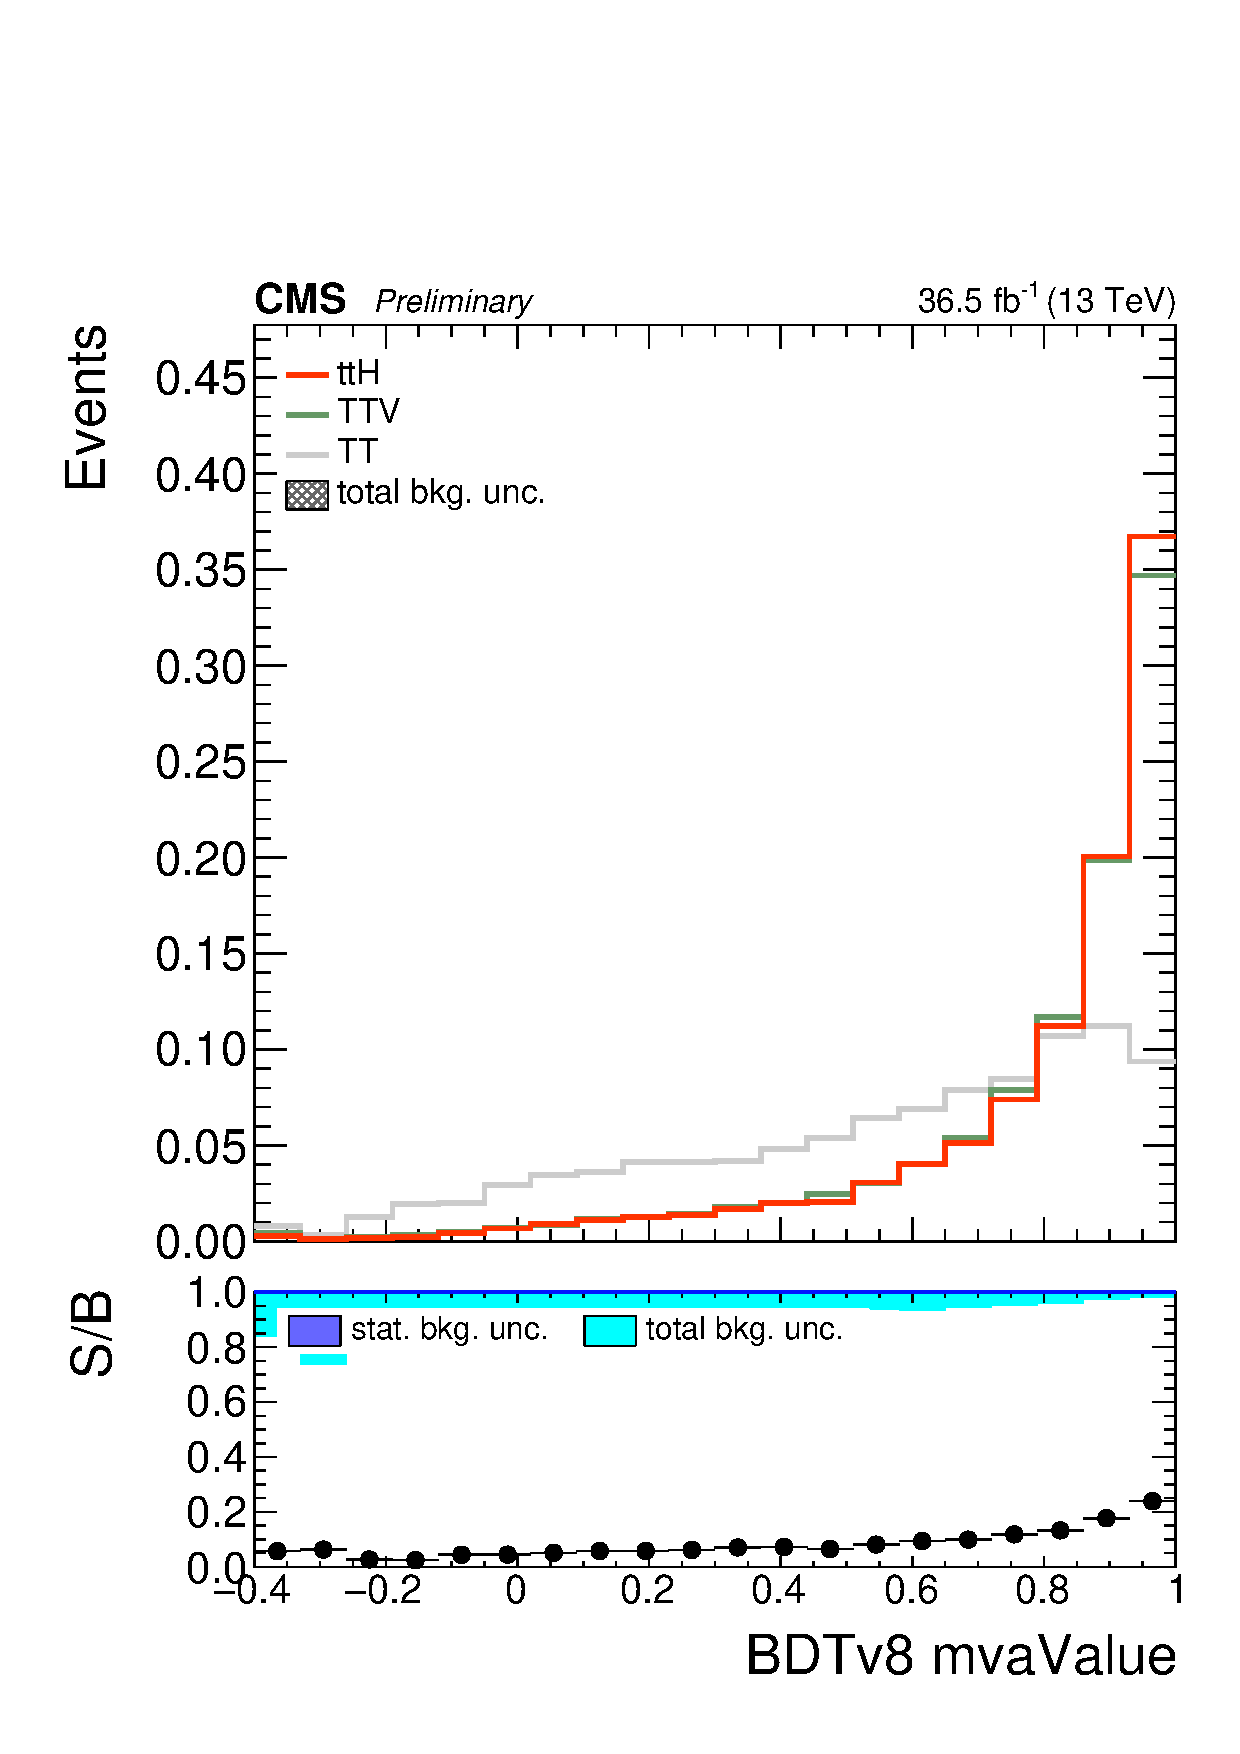
\includegraphics[width=0.3\textwidth]{ch9_figs/kinMVA_input_BDTv8_eventReco_mvaValue.pdf}
\caption[Signal extraction BDT input variables]{Separtion power among various backgrounds for BDT input variables}
\label{fig:inputs2.5}
\end{figure}

\begin{figure}[htp]
\centering
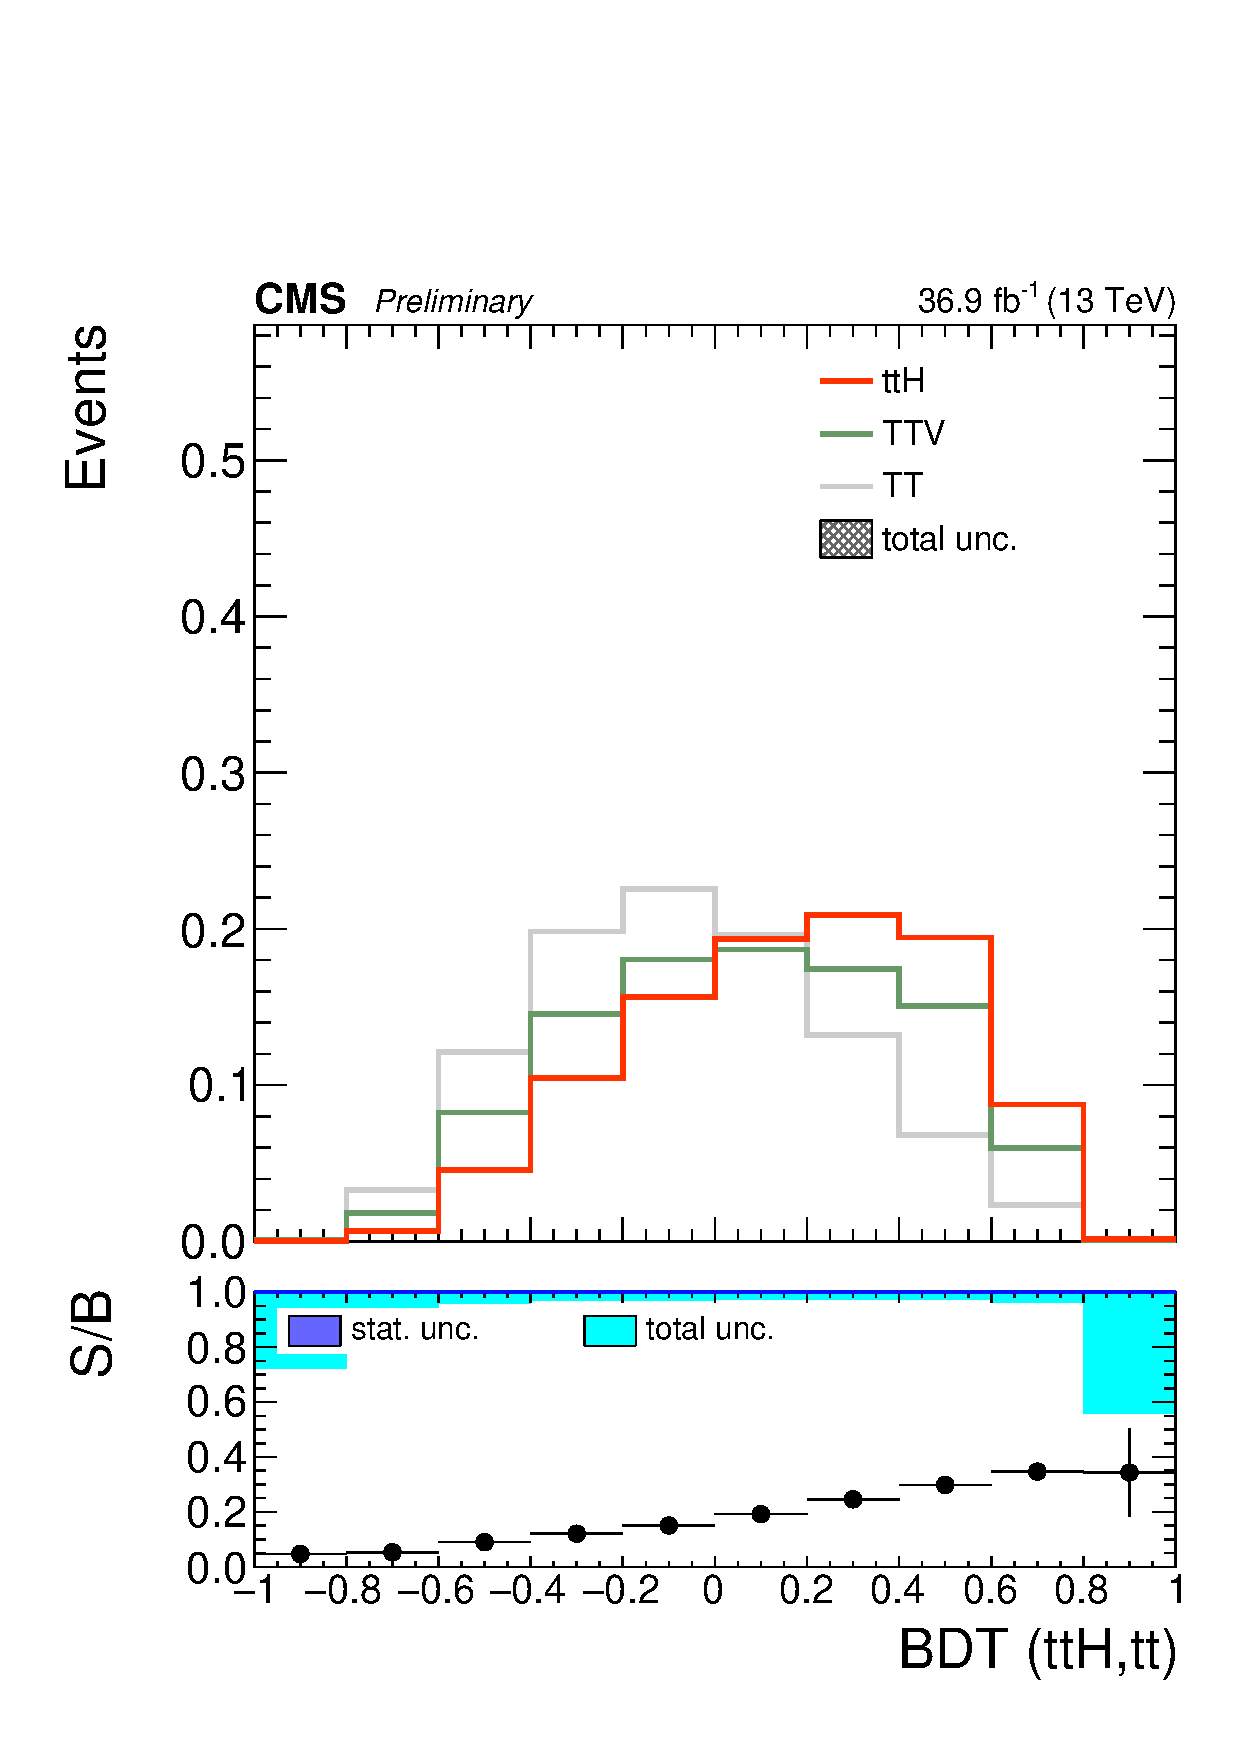
\includegraphics[width=0.49\textwidth]{ch9_figs/kinMVA_2lss_ttbar.pdf}
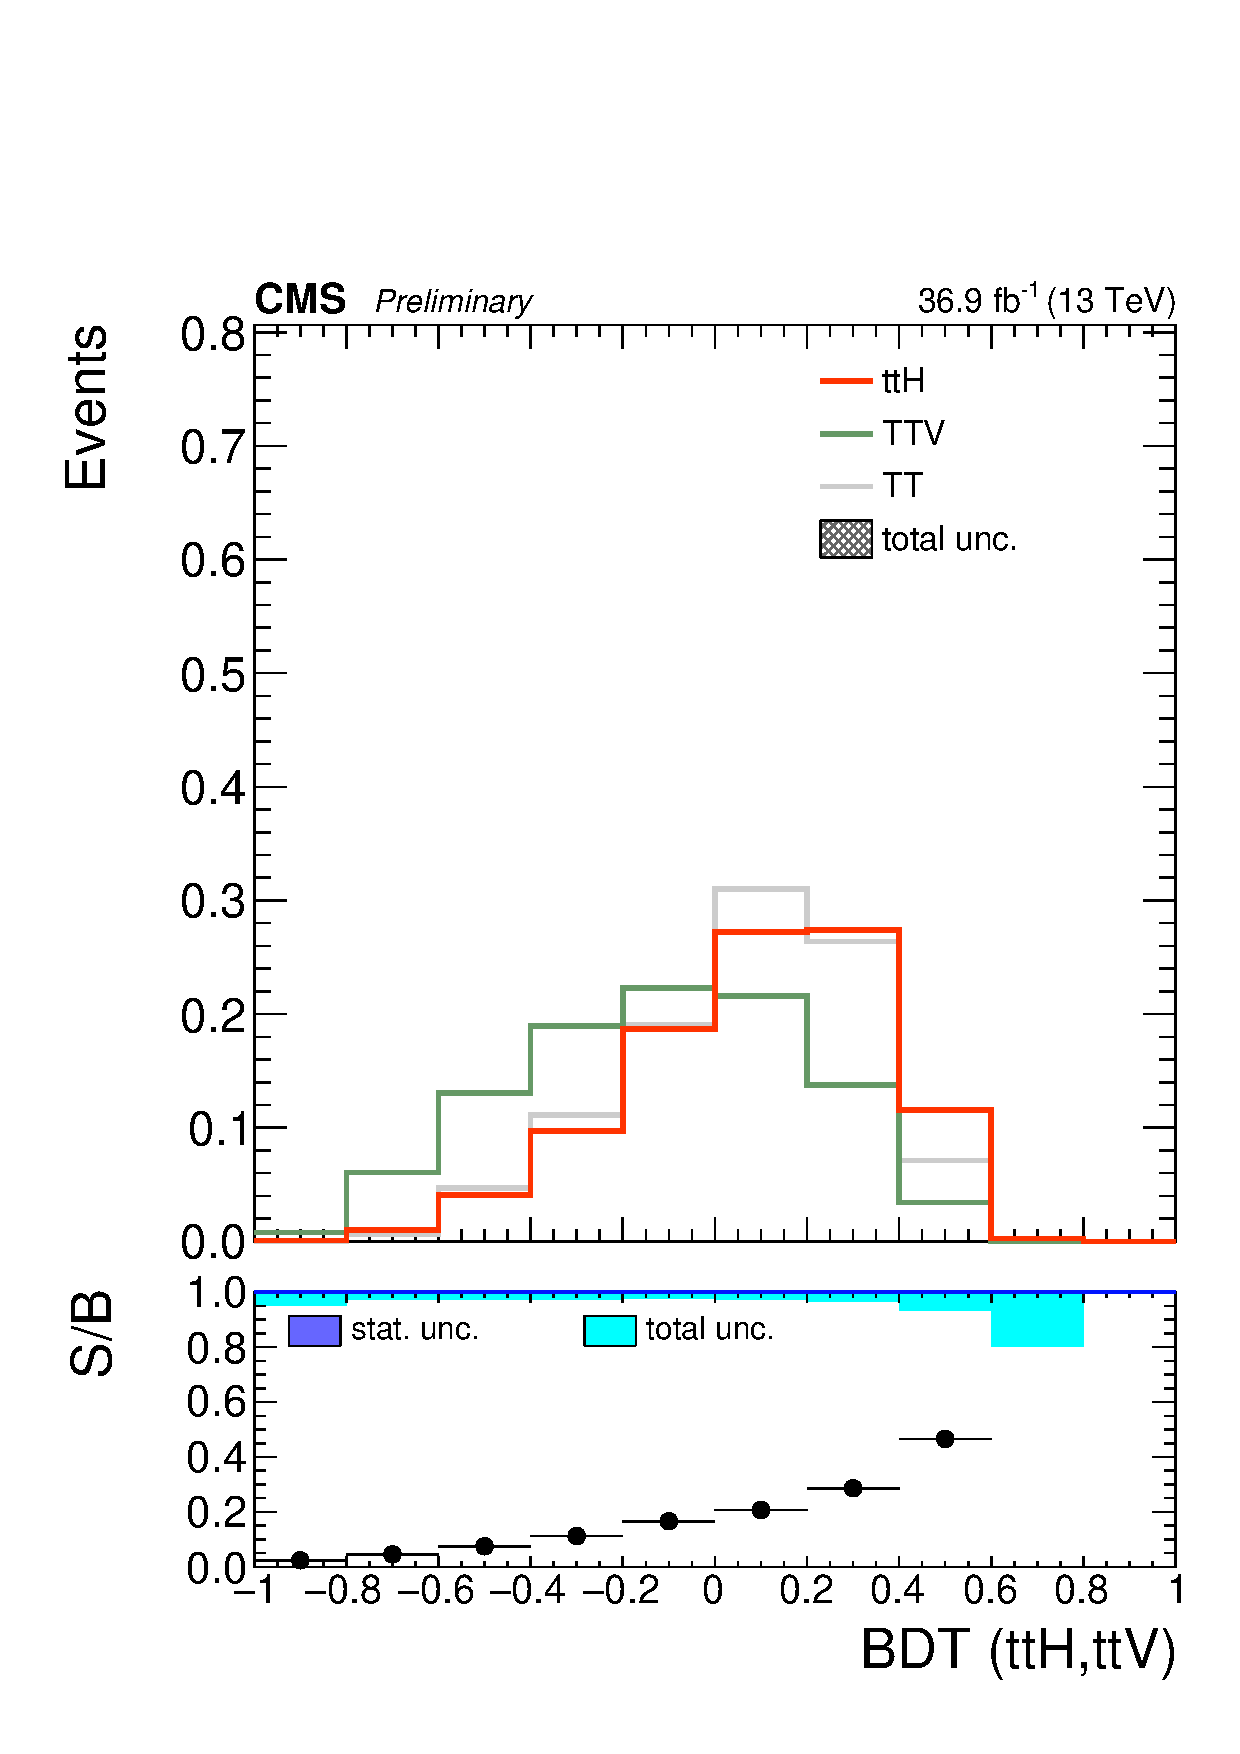
\includegraphics[width=0.49\textwidth]{ch9_figs/kinMVA_2lss_ttV.pdf}\\
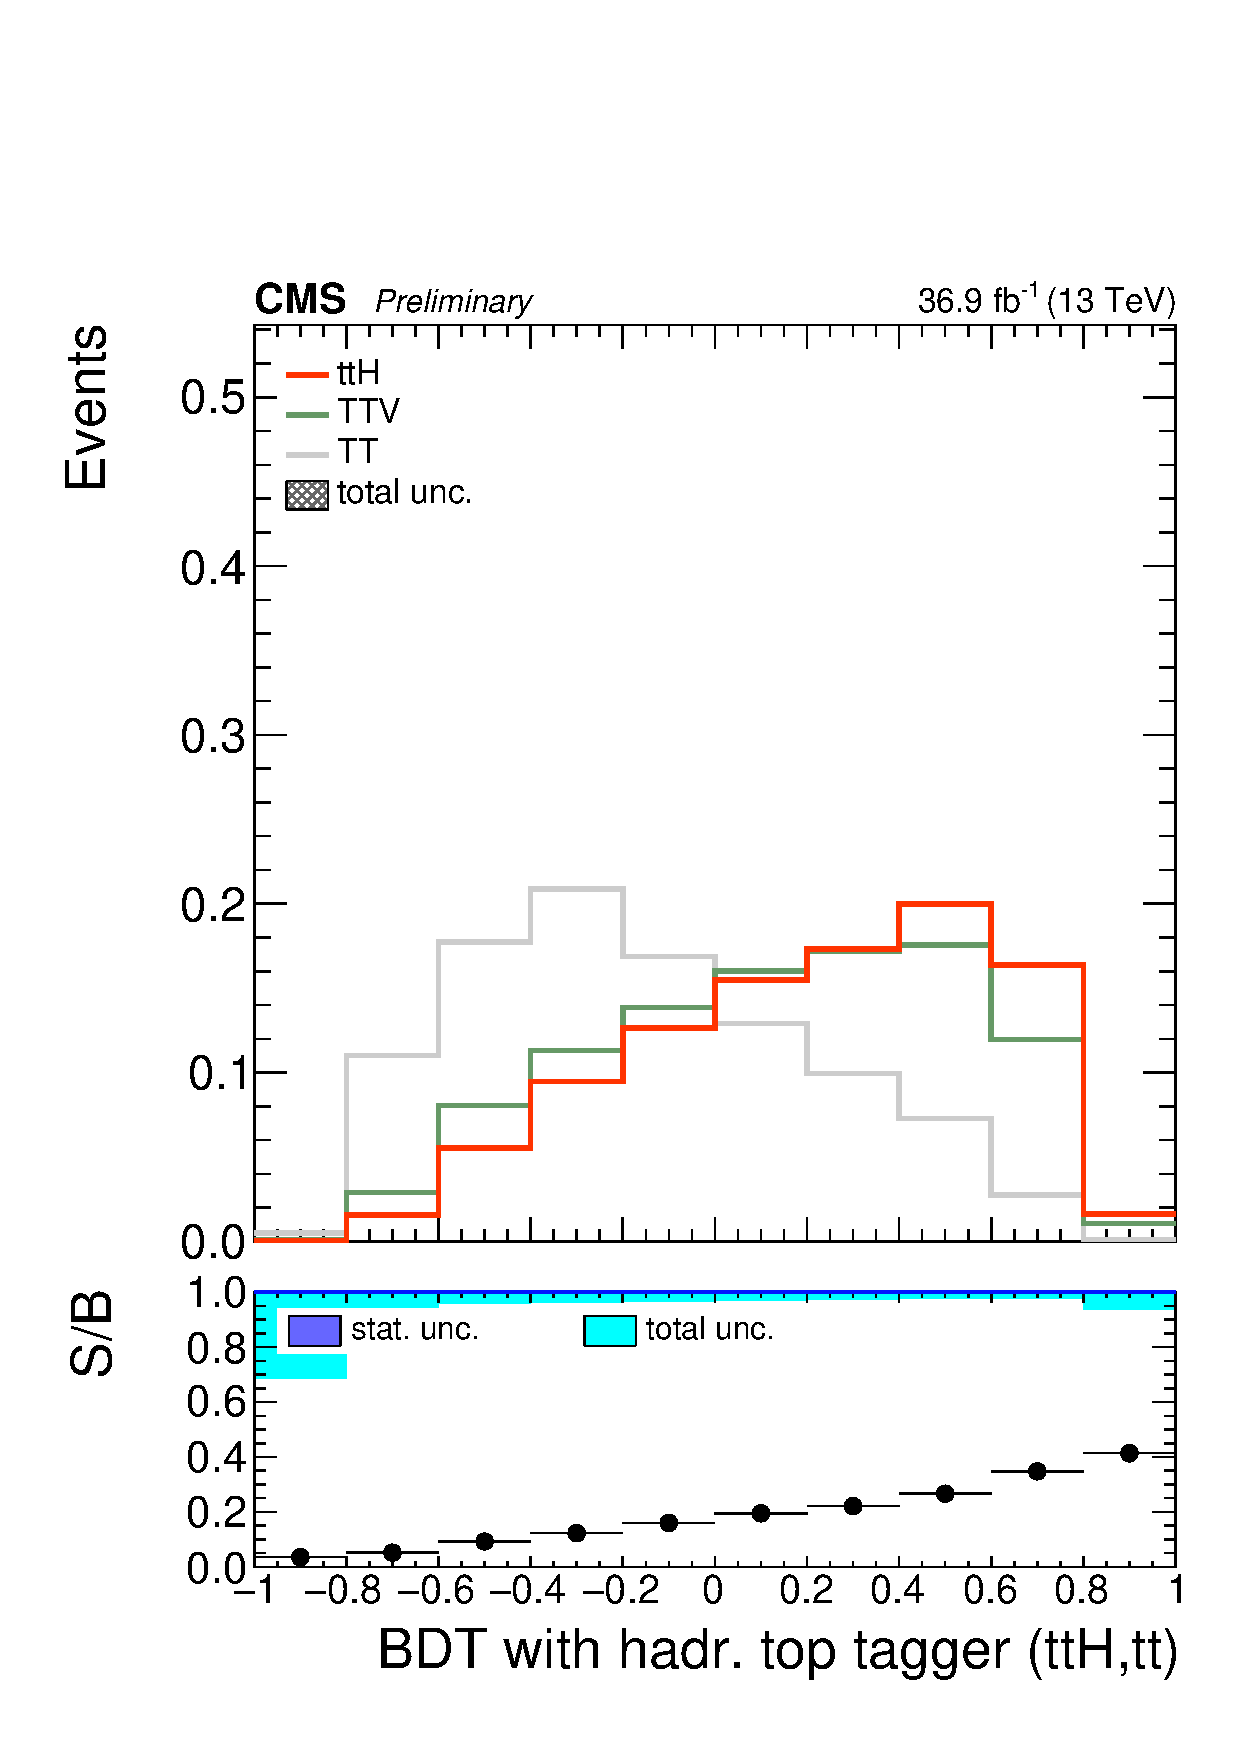
\includegraphics[width=0.49\textwidth]{ch9_figs/kinMVA_2lss_ttbar_withBDTv8.pdf}
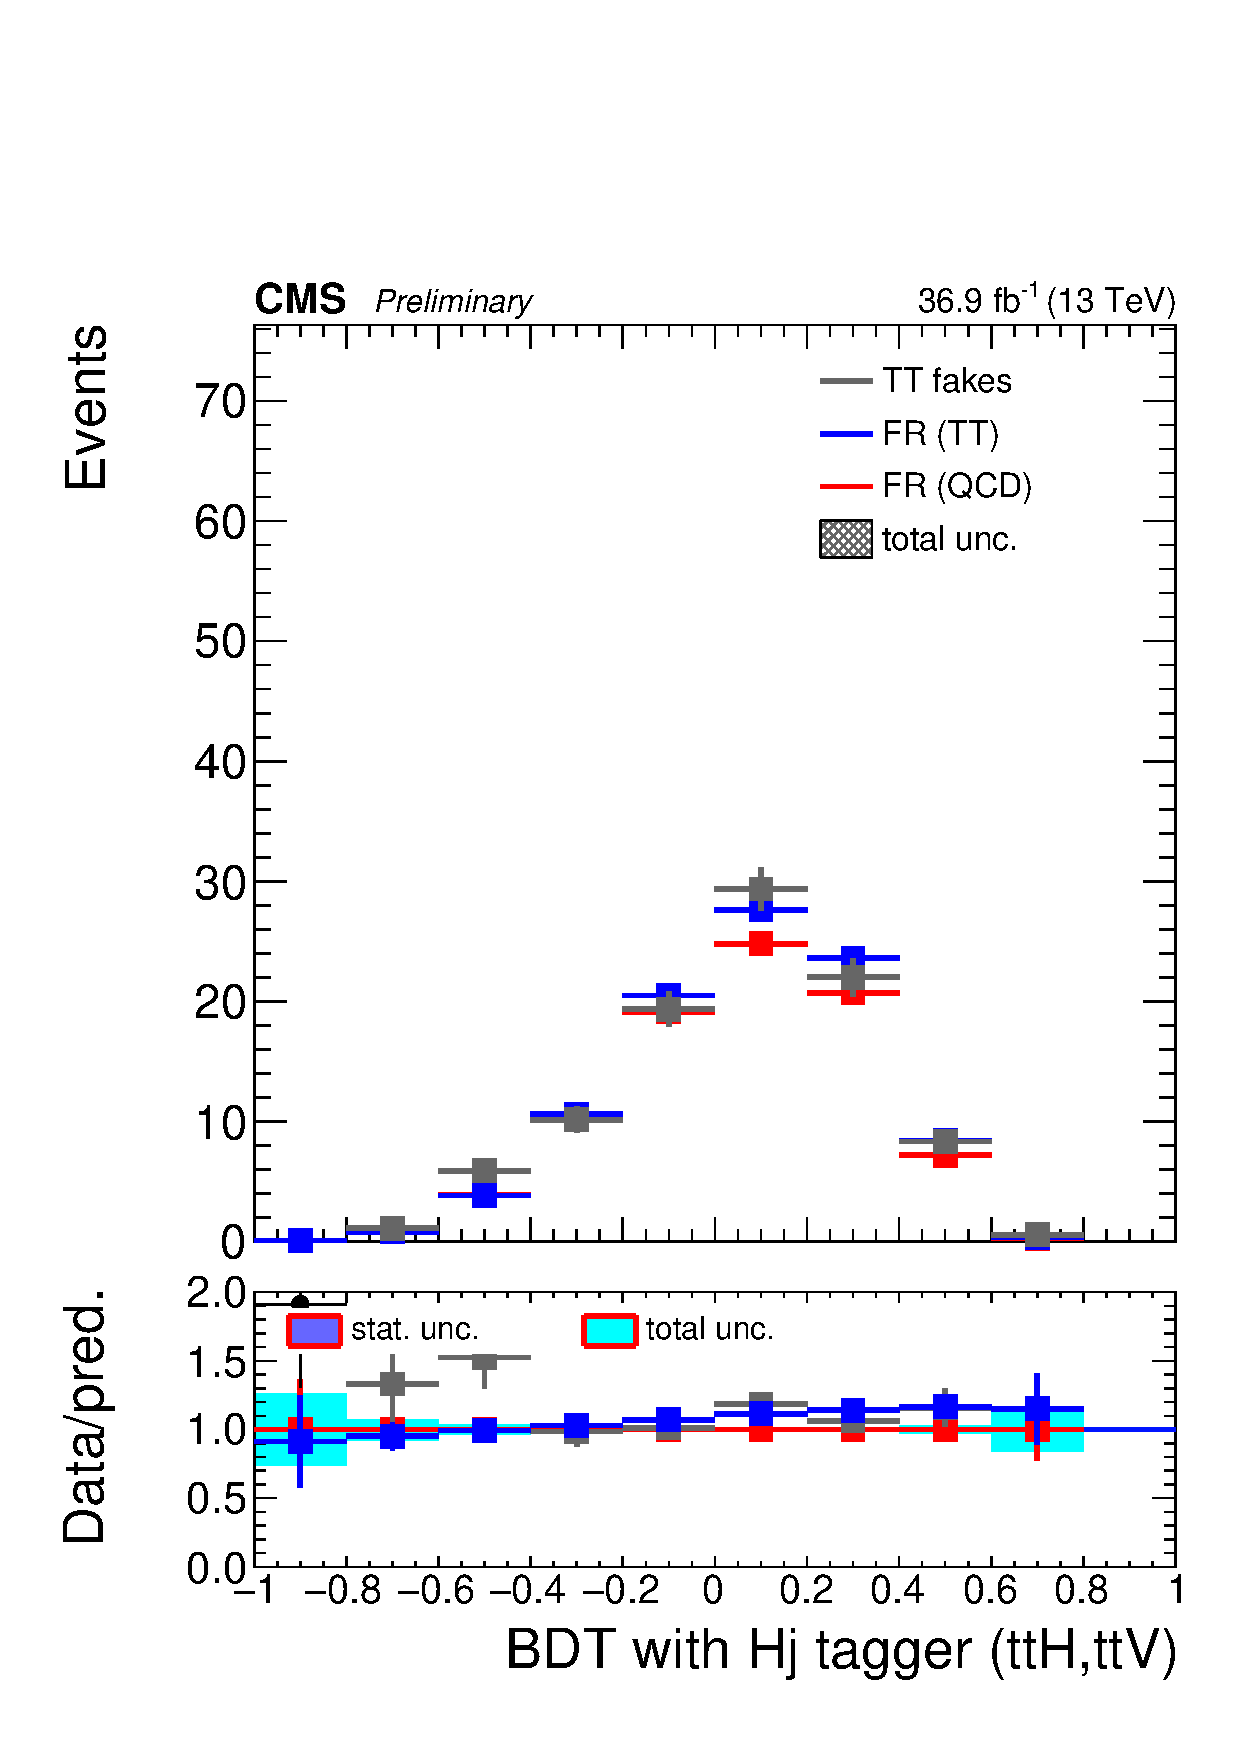
\includegraphics[width=0.49\textwidth]{ch9_figs/kinMVA_2lss_ttV_withHj.pdf}
\caption[BDT output scores with and without reconstruction inputs]{The BDT output scores without the reconstruction inputs (top) and with (bottom).}
\label{fig:inputs3}
\end{figure}

\subsection{Hadronic Top Reconstruction}
The reconstruction of the hadronic top decay is performed with a BDT. The objective is to correctly match
each selected jet and lepton to a final state particle in a $t\bar{t}H$ event, then
use the BDT response and other variables from the reconstruction to discriminate
against events without a hadronic top.     

Event reconstruction targets the 2lss category, specifically where the Higgs decays
to $W$ bosons. In the 2lss category, this means that one lepton originates from the
top system, and the other from the Higgs. For the jets, one of the
$W$ bosons from the Higgs decays hadronically, and one of the top quarks decays
hadronically, producing a total of two b-jets, and four light-flavor jets
from the hadronic $W$ decays. This specific decay is depicted by the diagram in Figure~\ref{fig:intro_feyn}.   

\subsubsection{Training}
The event reconstruction BDT is trained using the $t\bar{t}H$ monte-carlo powheg
signal sample used in training the final discrimination BDTs described previously.

The signal is gen-matched $t\bar{t}H$ events, which pass the same loosened training selection
described in Section~\ref{sec:2D_BDT}, with one important difference. In the selection used
here, the same-sign requirement on the leptons is dropped. This doubles the amount of events available
for training and the gen-matching requirement ensures the signal kinematics are left unaffected. 
Because the 2lss event selection requires at least four jets, the vast majority of signal
events used for training are only partially reconstructed, since a full reconstruction
necessitates six matched jets. Because so few events can be fully reconstructed, we must
consider partial reconstructions for events that have fewer than six matched jets.
The strategy for this is to use ``null'' jets whose four-vectors are set to zero to
represent missing jets in the event. Finally we require the signal events to have two
correctly-matched selected leptons, and at least four correctly-matched selected jets.

The background consists of all jet and lepton permutations of incorrectly-matched
$t\bar{t}$ events. This means that in each background event, there must be at least one
object that is incorrectly matched. For example when considering the object-matching to the
leptonically decaying top quark, a background training event where the reco-level jet assigned
to the b-jet, is actually the b-jet at gen-level, the reco-level lepton must originate from some source
other than the W from the leptonically decaying top. In this way, a single \ttbar MC
background event is used multiple times, once for each distinct permutation of 6 objects, in the training.
It was found that this technique produces far more background 


For the background, the null jets are added according to the
jet multiiplicity. For events with seven or fewer selected jets, three null jets are
added, for events with eight selected jets, two null jets are added, and one null jet
is added for events with greater than eight selected jets. The motiviation for this recipe
comes from a study of \tth events in the signal region comparing the number of reco jets that are
gen-matched to the \tth process, with the jet multiplicity in the event. The results of this study are
in Figure~\ref{fig:jet_matching}. 

\begin{figure}[htp]
\centering
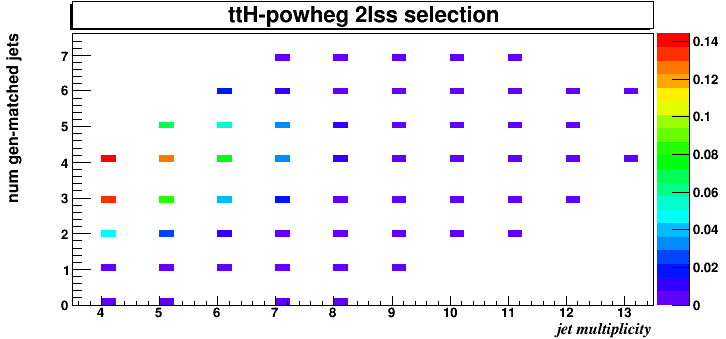
\includegraphics[width=0.49\textwidth]{ch9_figs/jet_matching.png}
\caption[Comparison of gen-matched jet multiplicity to jet multiplicity in signal events]{ Normalized histogram of gen-matched jet multiplicity vs jet multiplicity in \tth MC in the signal region.}
\label{fig:jet_matching}
\end{figure}

To reduce the computation time and improve performance,
several cuts are applied at each permutation to remove unlikely reconstructions.
These cuts include applying the b-tag requirement on the two jets being considered
as b-jets (1 b-tight OR 2 b-loose) described earlier, requiring that no
reconstructed $W$ have a mass greater than 120 GeV, requiring the leptonic top mass
be less than 180 GeV, and requiring 
the hadronic top mass be less than 220 GeV. Additionally, we ignore permutations
arising from swapping two light flavor jets from the same $W$ boson, as the reconstruction is
identical. An additional measure is taken to reduce permutation iterations, in the training step only,
which samples randomly from the available permutations in each event before the phyics-motivated cut is applied.
For each of the 8 objects, the permutation for that object skipped randomly 3 out of 10 times. For 8 objects,
this means that $0.7^{8} \approx 0.06$ or just 6$\%$ of the permutations for a given event are considered. After factoring
in the permutations skipped due to physics cuts, this number is even smaller. 

The BDT uses eight input variables, consisting of:
\begin{itemize}
\item The CSVv2 score of the b-jet assigned to the hadronic top
\item The CSVv2 score of the b-jet assigned to the leptonic top
\item The transverse momentum of the reconstructed hadronic top
\item The mass of the reconstructed hadronic top
\item The mass of the $W$ boson from the hadronic top
\item The transverse momentum ratio of the lepton from the Higgs to the lepton from the leptonic top
\item The solid angle between the lepton from the leptonic top and the b-jet from the hadronic top
\item The solid angle between the lepton from the leptonic top and the b-jet from the leptonic top
\item The solid angle between the lepton from the Higgs and the b-jet from the leptonic top
\end{itemize}

\noindent This approach focuses on the hadronic top decay, as the other aspects of the event
are more difficult to reconstruct due to the missing energy from the neutrinos. 

\subsubsection{Evaluation}

The event reconstruction BDT is evaluated by iterating over all possible lepton and jet
permutations, and selecting the highest scoring permutation as the reconstruction for
each event. For this evaluation, the null jet prescription and permutation
cuts used are identical to the background training.
The reconstruction is designed identify events that have a hadronic top present and
discriminates against the semi-leptonic $t\bar{t}$ background. The addition of the 
reconstruction BDT output as an input to the BDT targeting the $t\bar{t}$ background,
improves the performance by 10$\%$ by comparing ROC integrals when evaluated on $t\bar{t}$ MC and compared to the
equivalent BDT in the 2016 \tth ICHEP analysis~\cite{CMS-AN-16-022} that did not use this
as an input. These performance ROC curves are below in Figure~\ref{fig:hadtop_performance}.

\begin{figure}[htb]
 \centering
   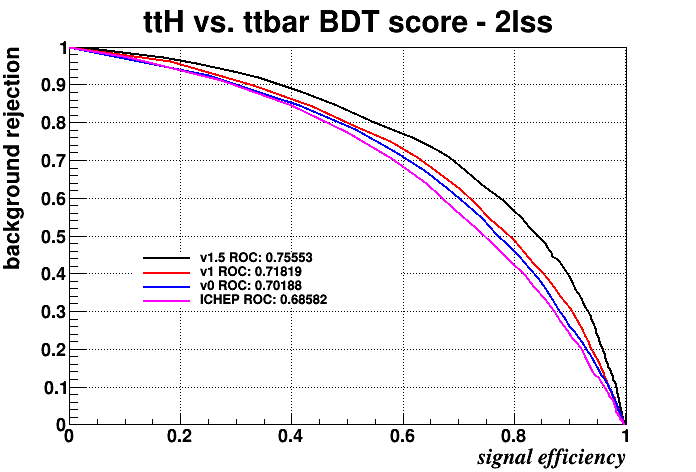
\includegraphics[width=0.6\textwidth]{ch9_figs/improvement_roc.png}
   \caption[ROC curves of $t\bar{t}$ BDT with and without hadronic top reconstruction input]{The ROC curves of the BDT targeting the $t\bar{t}$ background compared without 
   hadronic top reconstruction input (pink) to the version used in this analysis (black). The other curves represent incremental improvements to the hadronic top BDT. The signal
   and background on the x and y axes are \tth and \ttbar MC respectively. The improvement based on ROC integral by adding the hadronic top reconstruction score is 10$\%$.}
  \label{fig:hadtop_performance}
\end{figure}

\subsection{Higgs Jet Tagging}
The Higgs Jet (HJ) tagger is a BDT aimed specifically at identifying hadronic jets originating from the W bosons in \tth, H$\rightarrow$WW decays consistent
with the \tth diagram in Figure~\ref{fig:intro_feyn}. This decay topology is the most common of all \tth decays in the $2lss$ channel. This final state
consists of 2 b-quark jets, 4 hadronic (light flavor) jets, 2 same-sign leptons, and missing energy due to neutrinos. The signal region selection described
in Chapter~\ref{chap:event_selection} does not require all of these objects to be present, as some or many are often out of the acceptance. This means that
the jets from the Higgs decay could be missing entirely from the event.

The HJ tagger addresses both the complicated jet combinatorics associated with this final state, but also the reality that not all jets originating
from the Higgs are selected. The HJ tagger is an object-level discriminator that exploits jet kinematics and identification variables to estimate the likelihood
of a jet originating from the Higgs. Similar to the hadronic top reconstruction method, the HJ tagger calculates scores for every jet in each event, selecting
the highest score as the output. To boost performance and simplify the combinatorics associated with tagging, the hadronic top tagger is first run,
and the jets selected as being assocaited with the hadronic top are removed from further consideration by the HJ tagger.
The HJ tagger is primarily aimed at selected jets from W decays (from the Higgs) and is used as a discriminating varible against both the \ttw and \ttz backgrounds.
Both of these
backgrounds are very likely to contain most or all of the hadronic top decay products, namely a b-tagged jet and two light flavor jets. The two light flavor jets from
the W in the hadronic top decay look kinematically similar to the targeted jets from the W from the Higgs, creating a potential for Higgs jet mis-tagging. This is
especially true when the b-jet is missing. The hadronic top tagger idenifies these jets and they are removed from consideration by the HJ tagger.

The HJ tagger is trained on \tth and \ttv MC. The signal training events require the reco-level objects passing the selection to be matched to a generator-level parton
originating from the H$\rightarrow$WW$\rightarrow l\nu~l\nu$ process. The background selection requires \ttv events in the signal region.  
The input variables include:
\begin{itemize}
\item the minimum angular separation between the jet and one of the two leptons
\item the maximum angular separation between the jet and one of the two leptons
\item the jet transverse momenta
\item the jet b-tag discriminator (CSVv2)
\item the jet quark-gluon discriminator (qgid)
\end{itemize}

\noindent The qgid varible is a BDT designed to discriminate jets originating from light flavor quarks from jets originating from gluons. The performance and improvement due
to the HJ tagger input is seen in Figure~\ref{fig:hj_tagger}.

\begin{figure}[htp]
\centering
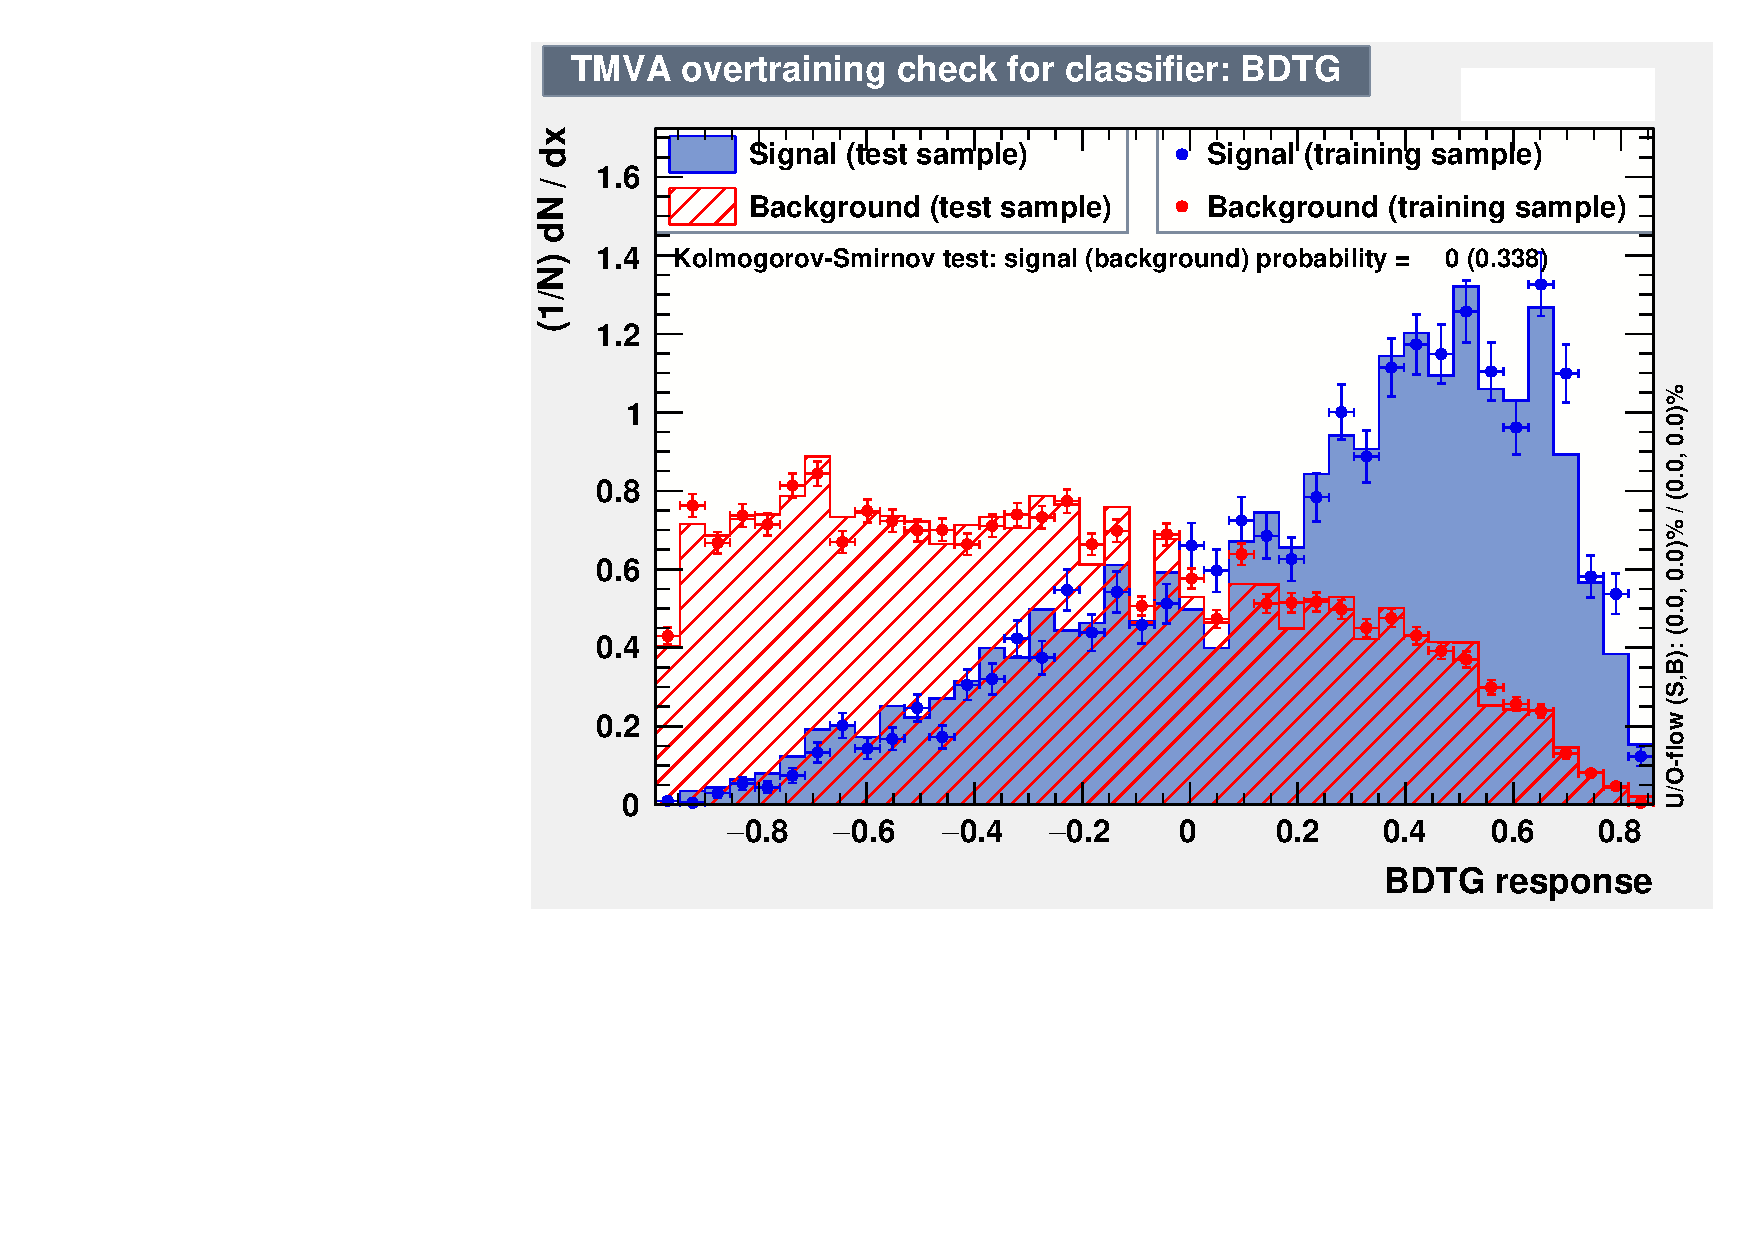
\includegraphics[width=0.49\textwidth]{ch9_figs/Jtagger_Ks.pdf}
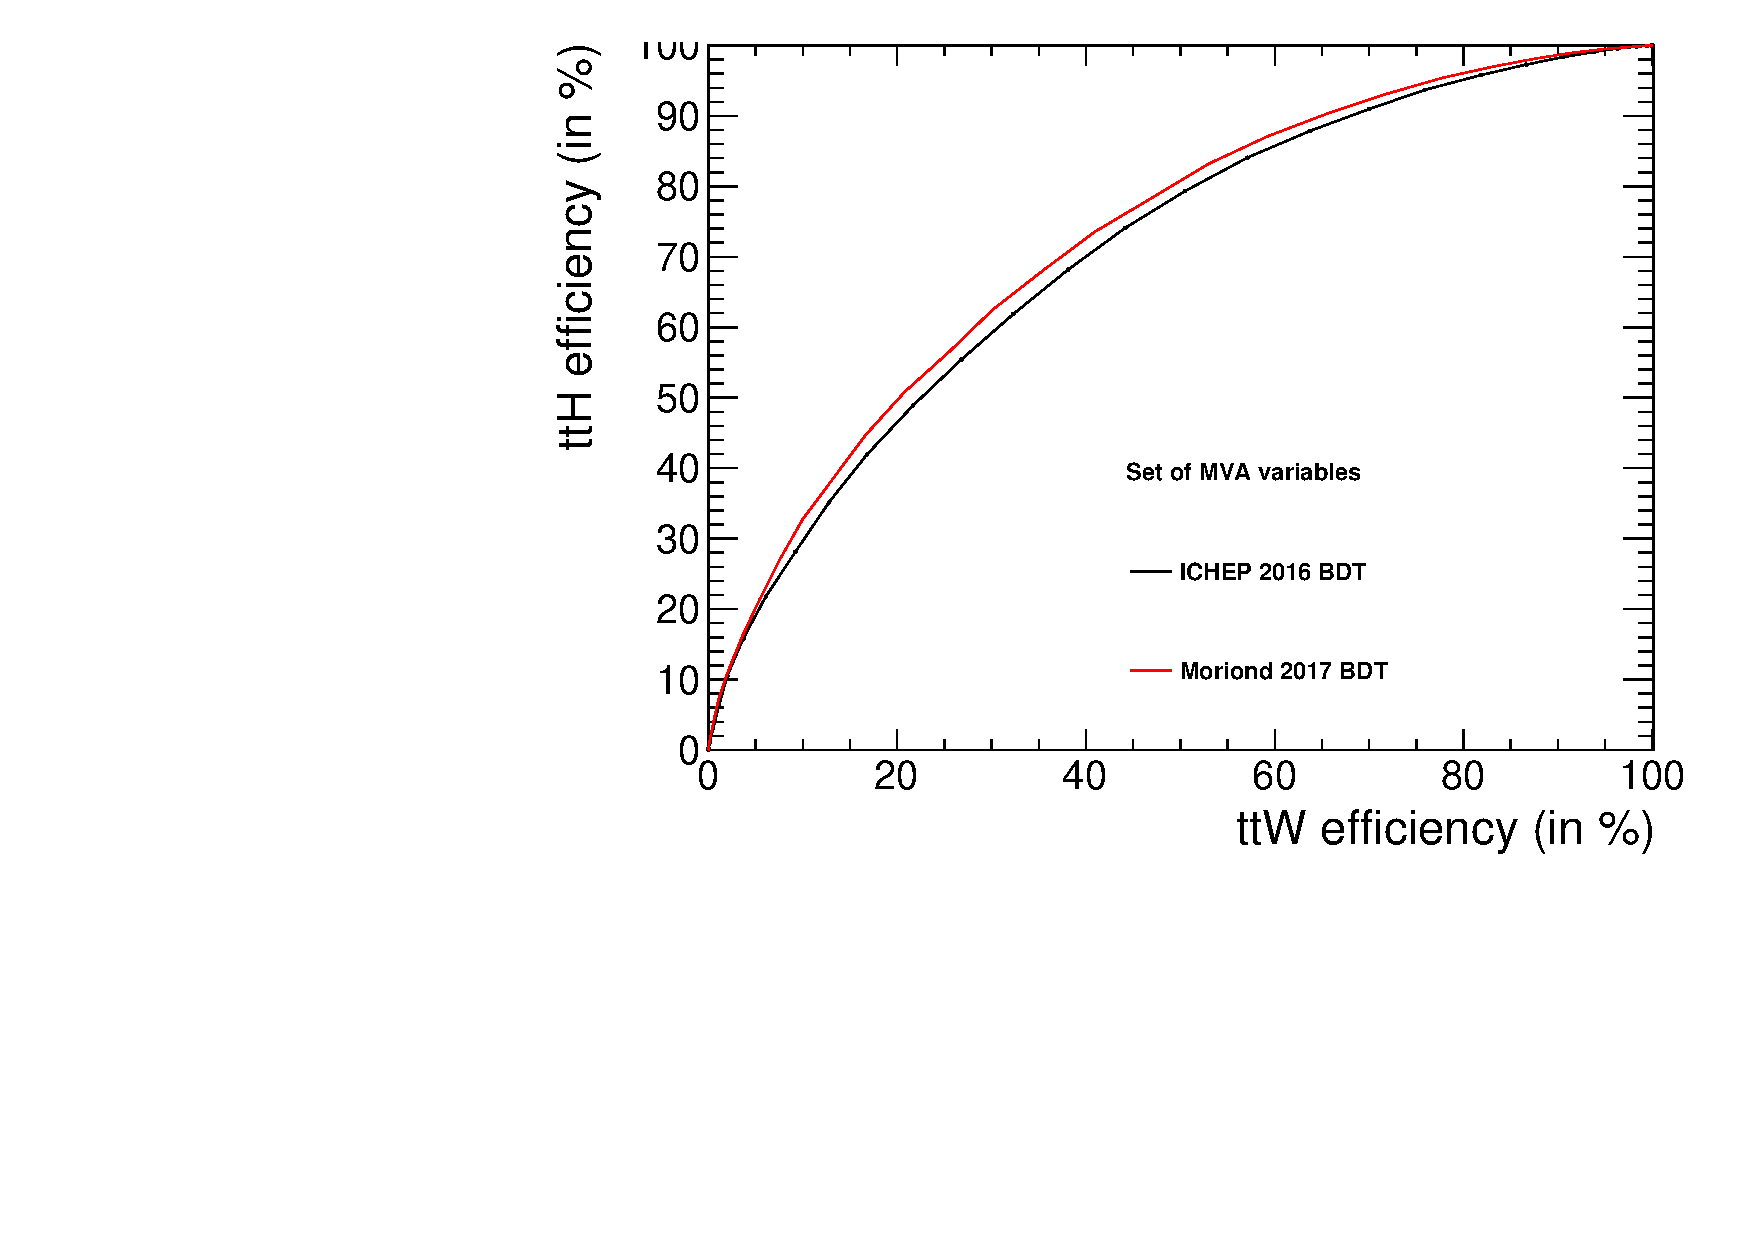
\includegraphics[width=0.49\textwidth]{ch9_figs/Roc_Comparison_18Feb.pdf}
\caption[Performance improvement from the HJ tagger and hadronic top removal]{Separation power of HJ output on the training samples (right) and performance improvements with respect to the 2016 version of this analysis obtained with the HJ
tagger input with hadronic top removal (left).}
\label{fig:hj_tagger}
\end{figure}

\section{Binning}
The binning choice for the two-dimensional shape resulting from plotting each BDT on a separate axis is not straight forward, since overlaying the shapes across signal and backgrounds is not possible.
The binning method must optimally partition the space to isolate
signal from background, while simultaneously maintaining populated bins that don't suffer from low statistics. The output shapes formed by the two BDTs for the signal and largest backgrounds
are in Figure~\ref{fig:2d_shapes} below. 

\begin{figure}[htp]
\centering
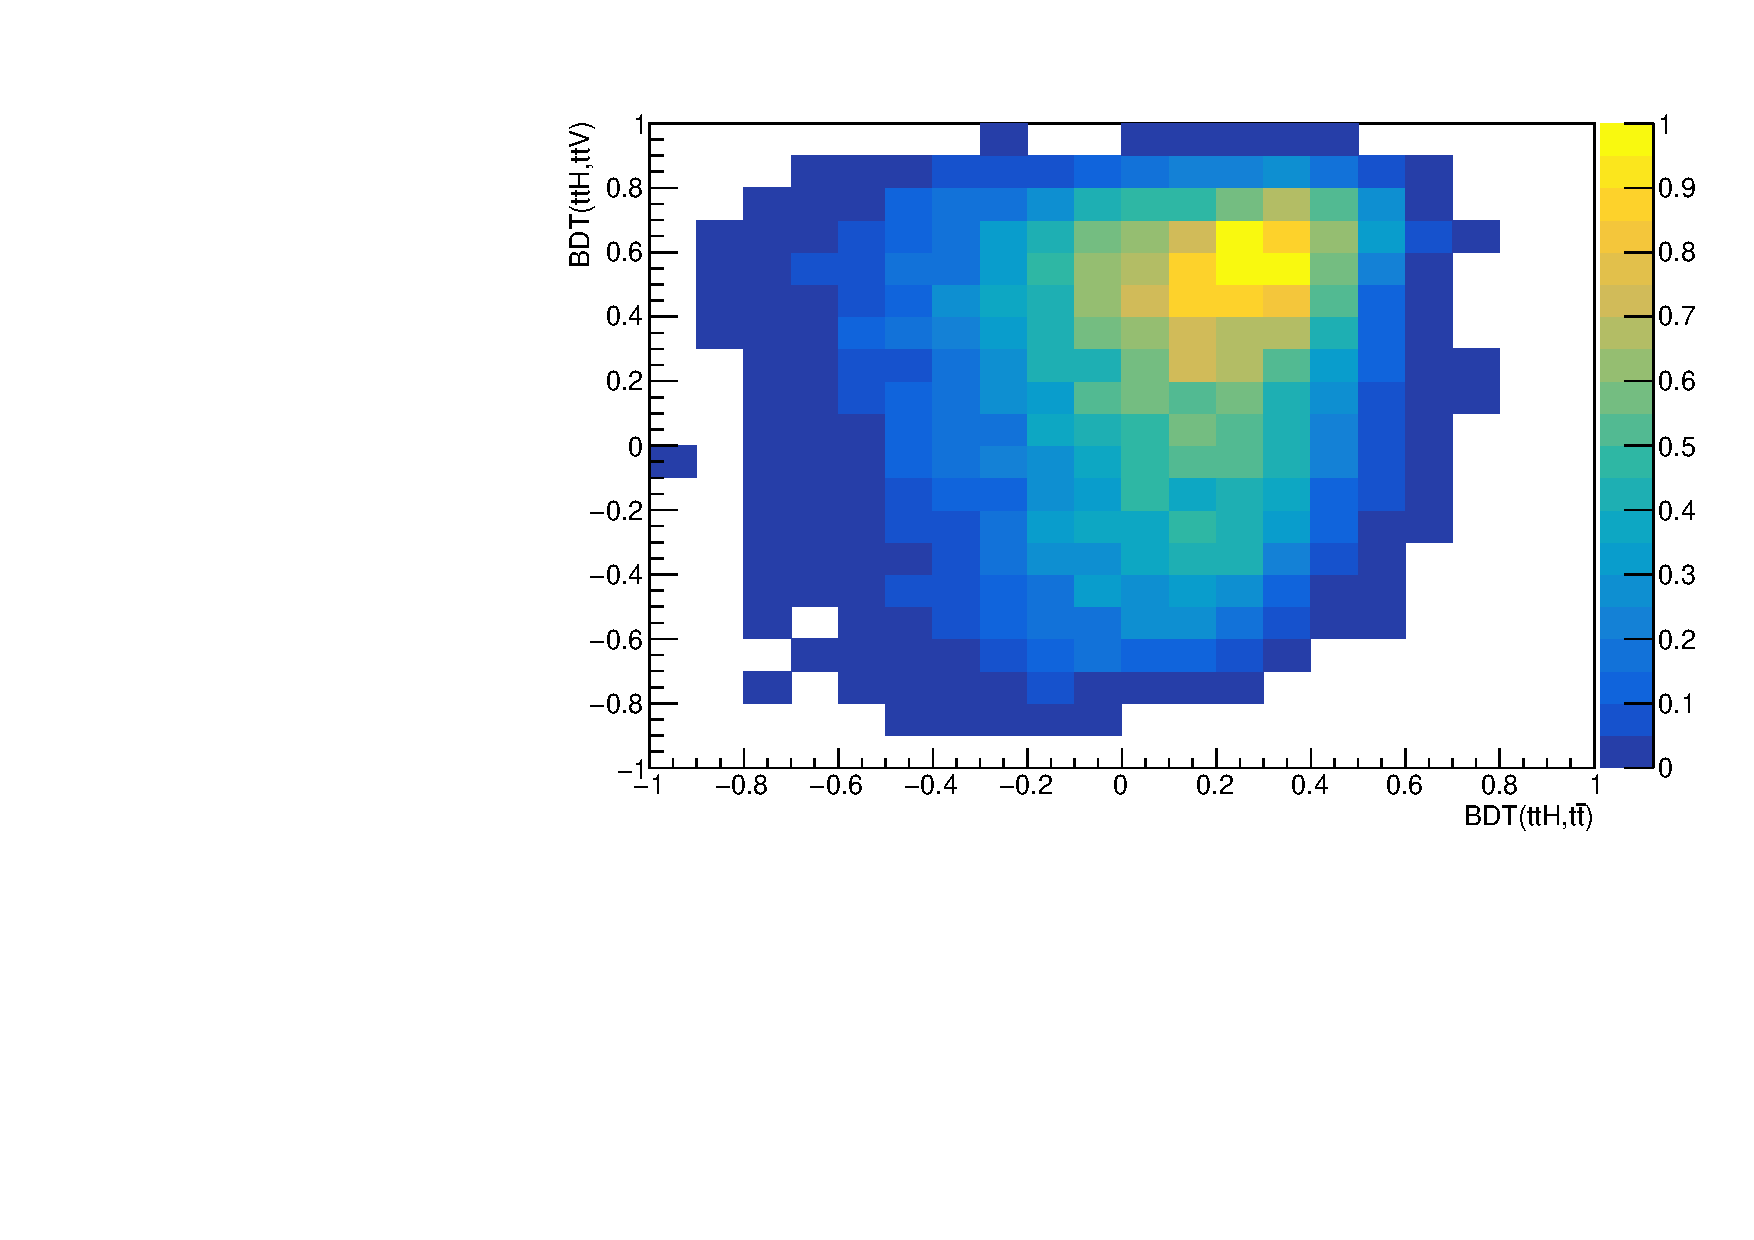
\includegraphics[width=0.49\textwidth]{ch9_figs/tth_2l_2D.pdf}\\
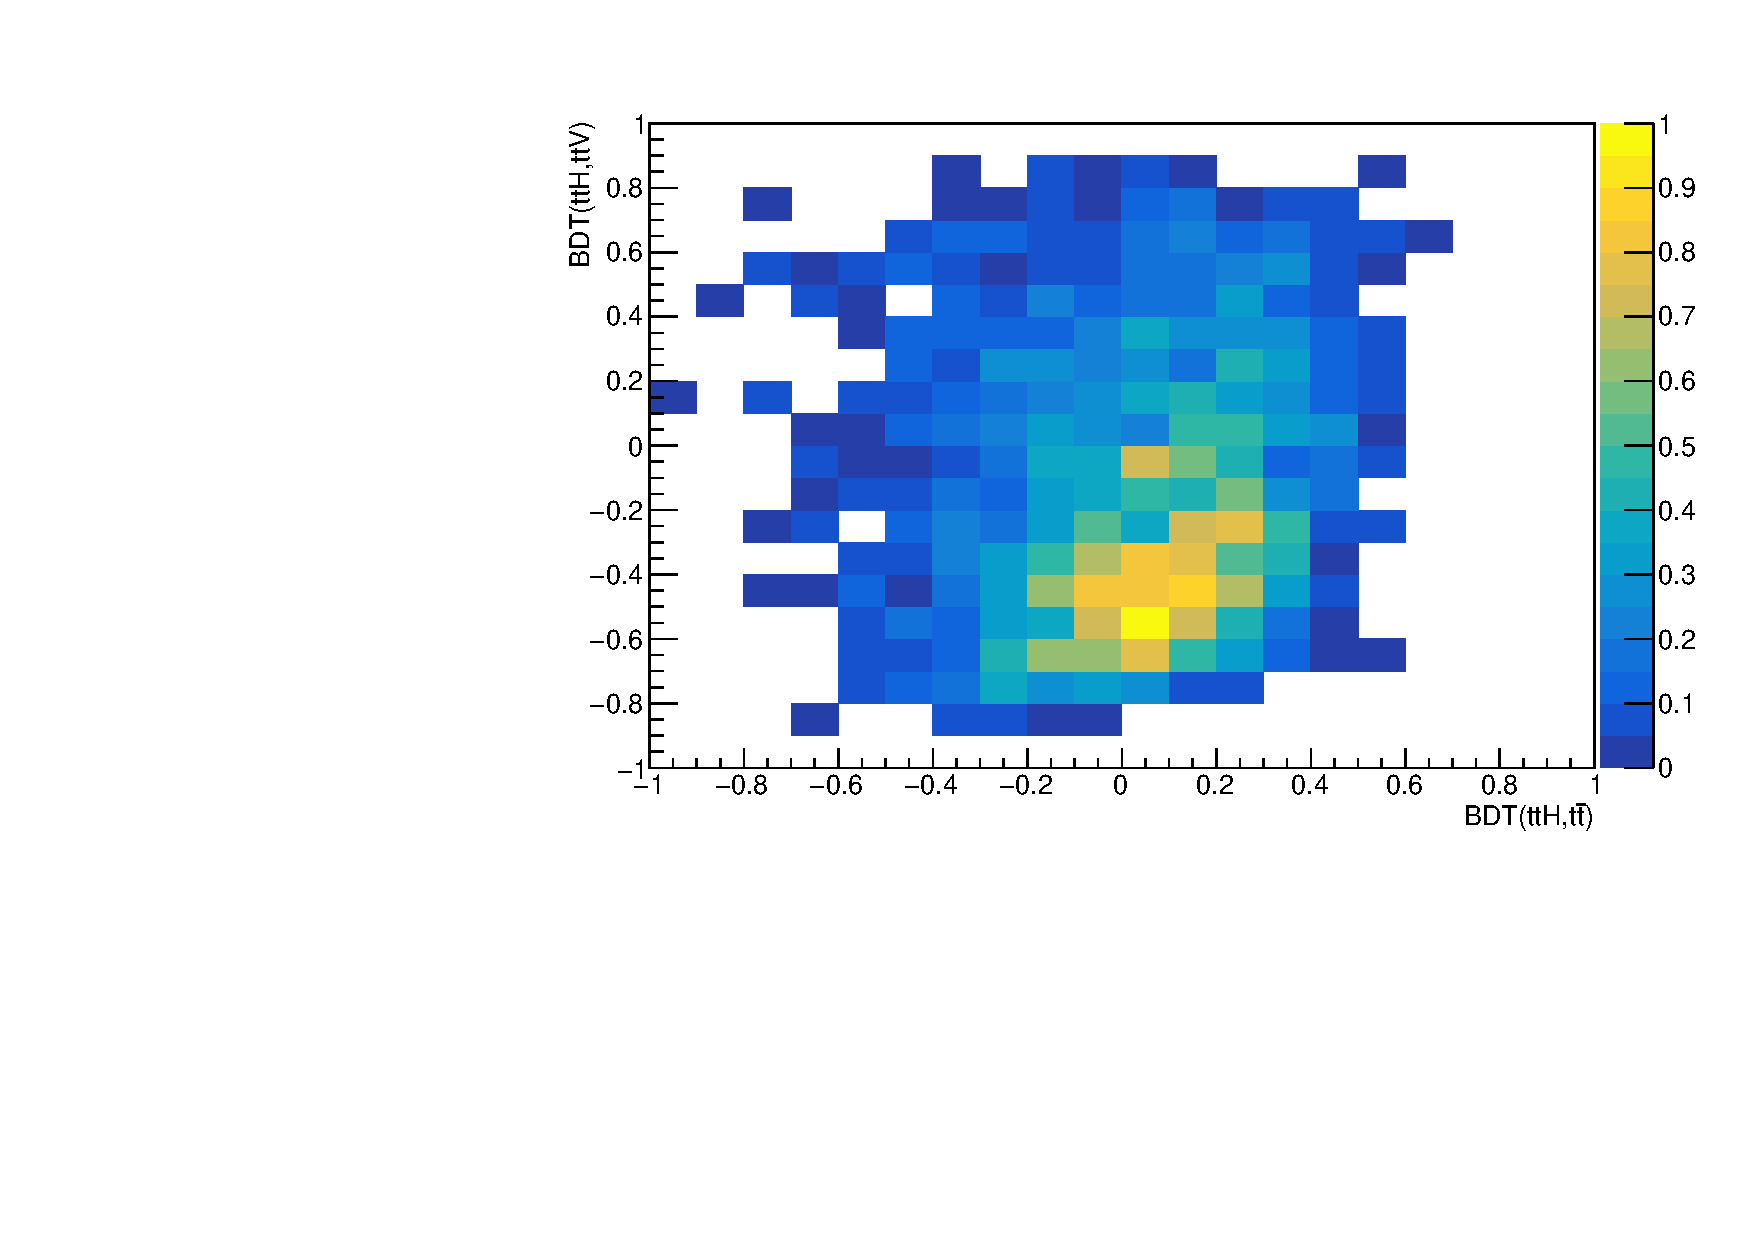
\includegraphics[width=0.49\textwidth]{ch9_figs/tt_2l_2D.pdf}
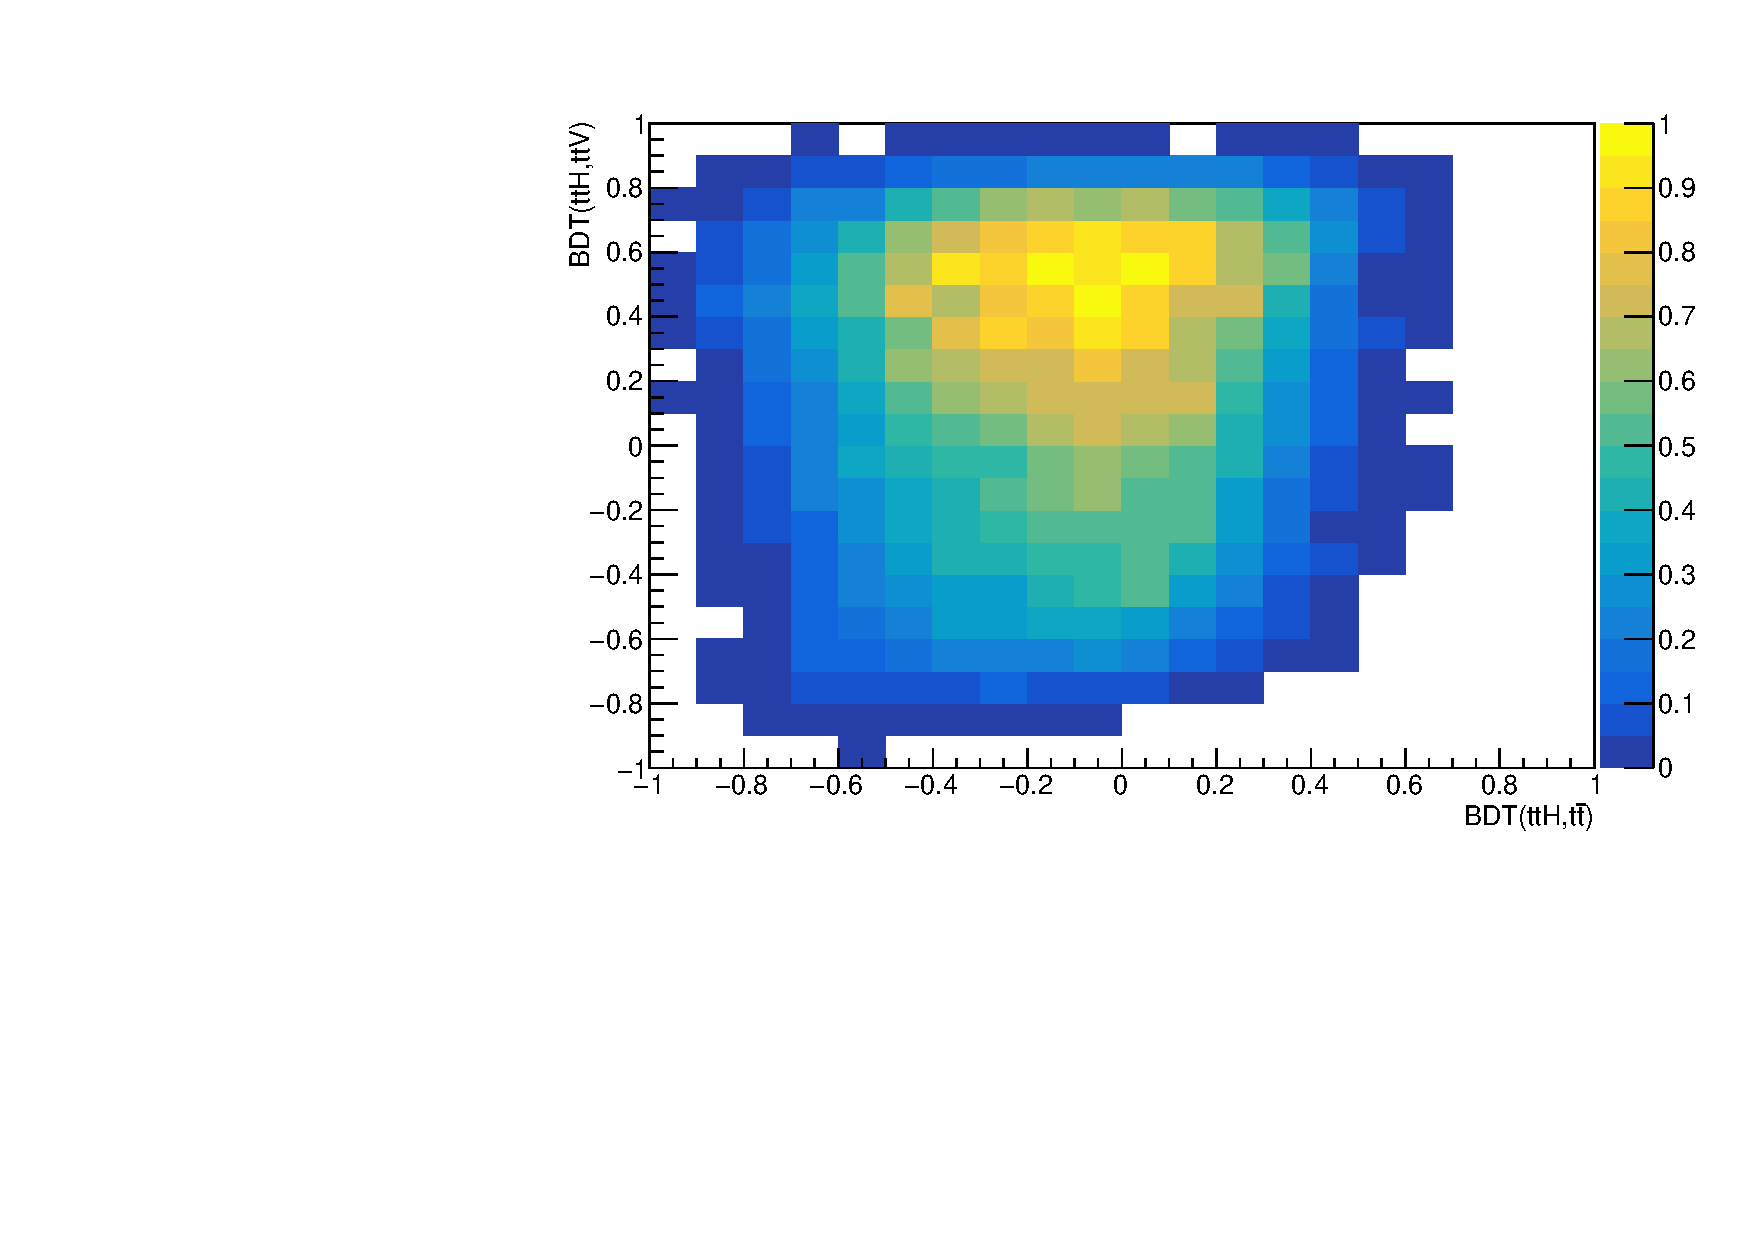
\includegraphics[width=0.49\textwidth]{ch9_figs/ttw_2l_2D.pdf}
\caption[Two dimensional BDT output shapes of signal and backgrounds]{The two-dimensional output shape formed by the two BDTs for \tth (top), \ttbar (left), and \ttv (right).}
\label{fig:2d_shapes}
\end{figure}

While previous versions of this analysis used a simple rectangular binning that was performed by studying the signal and background shapes and drawing the bins by hand,
this iteration takes a more scientific approach based on the signal-to-background likelihood ratio. The binning procedure was performed with signal and background MC that was not used
in the main analysis. The binning process begins with the standard rectangular, 20 x 20 binning in Figure~\ref{fig:2d_shapes}. For each bin, the signal to background likelihood ratio is computed.
Next, each background event from the \ttbar and \ttv samples is assigned the likelihood ratio corresponding to the bin it populates. The resulting likelihood distribution for background
events is transformed into the cumulative\footnote{A cumulative distribution function of some variable $S$, evaluated at $s$, is the probability that $S$ will have a value less than or equal
to $s$.} distribution below in Figure~\ref{fig:cum_dist} (left). The y-axis of the cumulative distribution function of background events is then binned evenly, achieving approximately equal
amounts of background in each bin.

\begin{figure}[htp]
\centering
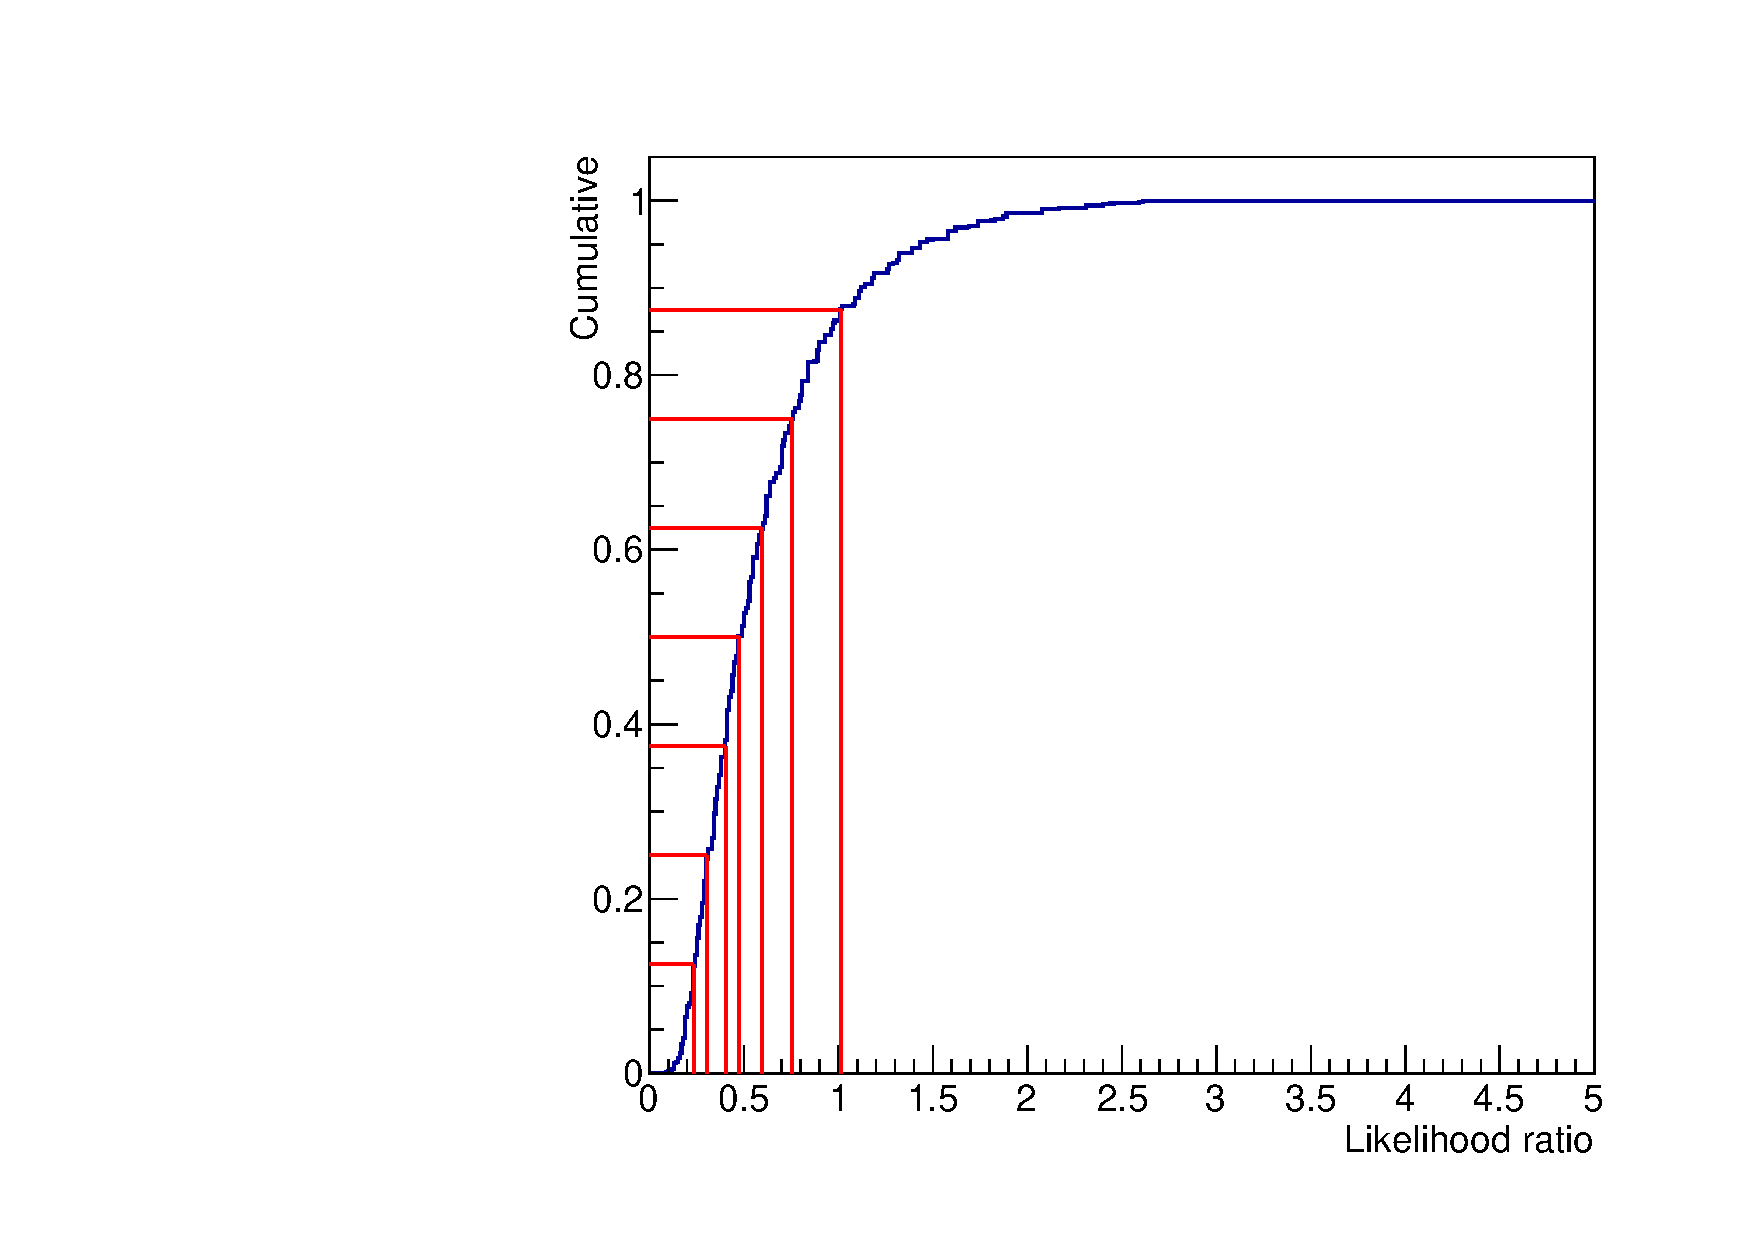
\includegraphics[width=0.49\textwidth]{ch9_figs/cumulative_2lss.pdf}
\caption[Cumulative distribution of signal-to-background likelihood ratio]{Cumulative distribution of signal-to-background likelihood ratio.}
\label{fig:cum_dist}
\end{figure}

\noindent The bins from the cumulative distribution are then mapped back to the 2D shape. This mapping is used as the final 2D binning and is represented in Figure~\ref{fig:likelihood} (left).
The corresponding 1D histogram resulting from this binning where the analysis is performed is Figure~\ref{fig:likelihood} (right). These bins are filled with separate signal and background
samples from the ones used for deriving final results. The choice of number of final bins is motived from a cross-check procedure based on the k-means algorithm, which yields similar
results~\cite{CMS-AN-17-029}. The pre-fit 1D shapes are in Figure~\ref{fig:final_shapes_prefit}. 

\begin{figure}[htp]
\centering
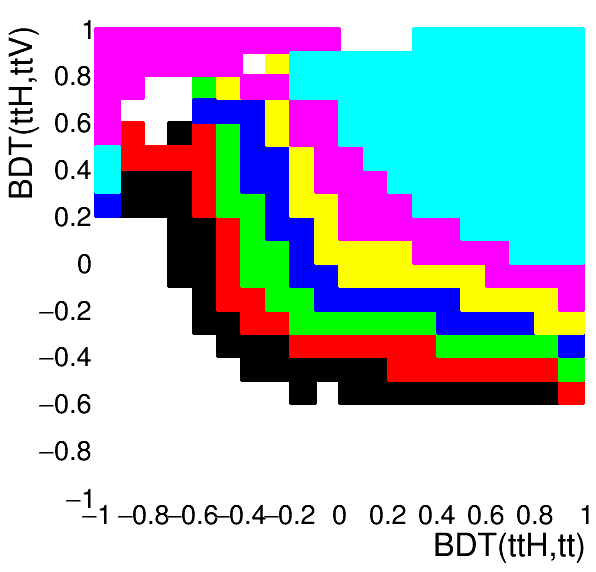
\includegraphics[width=0.49\textwidth]{ch9_figs/likelihoodBased_2d_2lss.png}
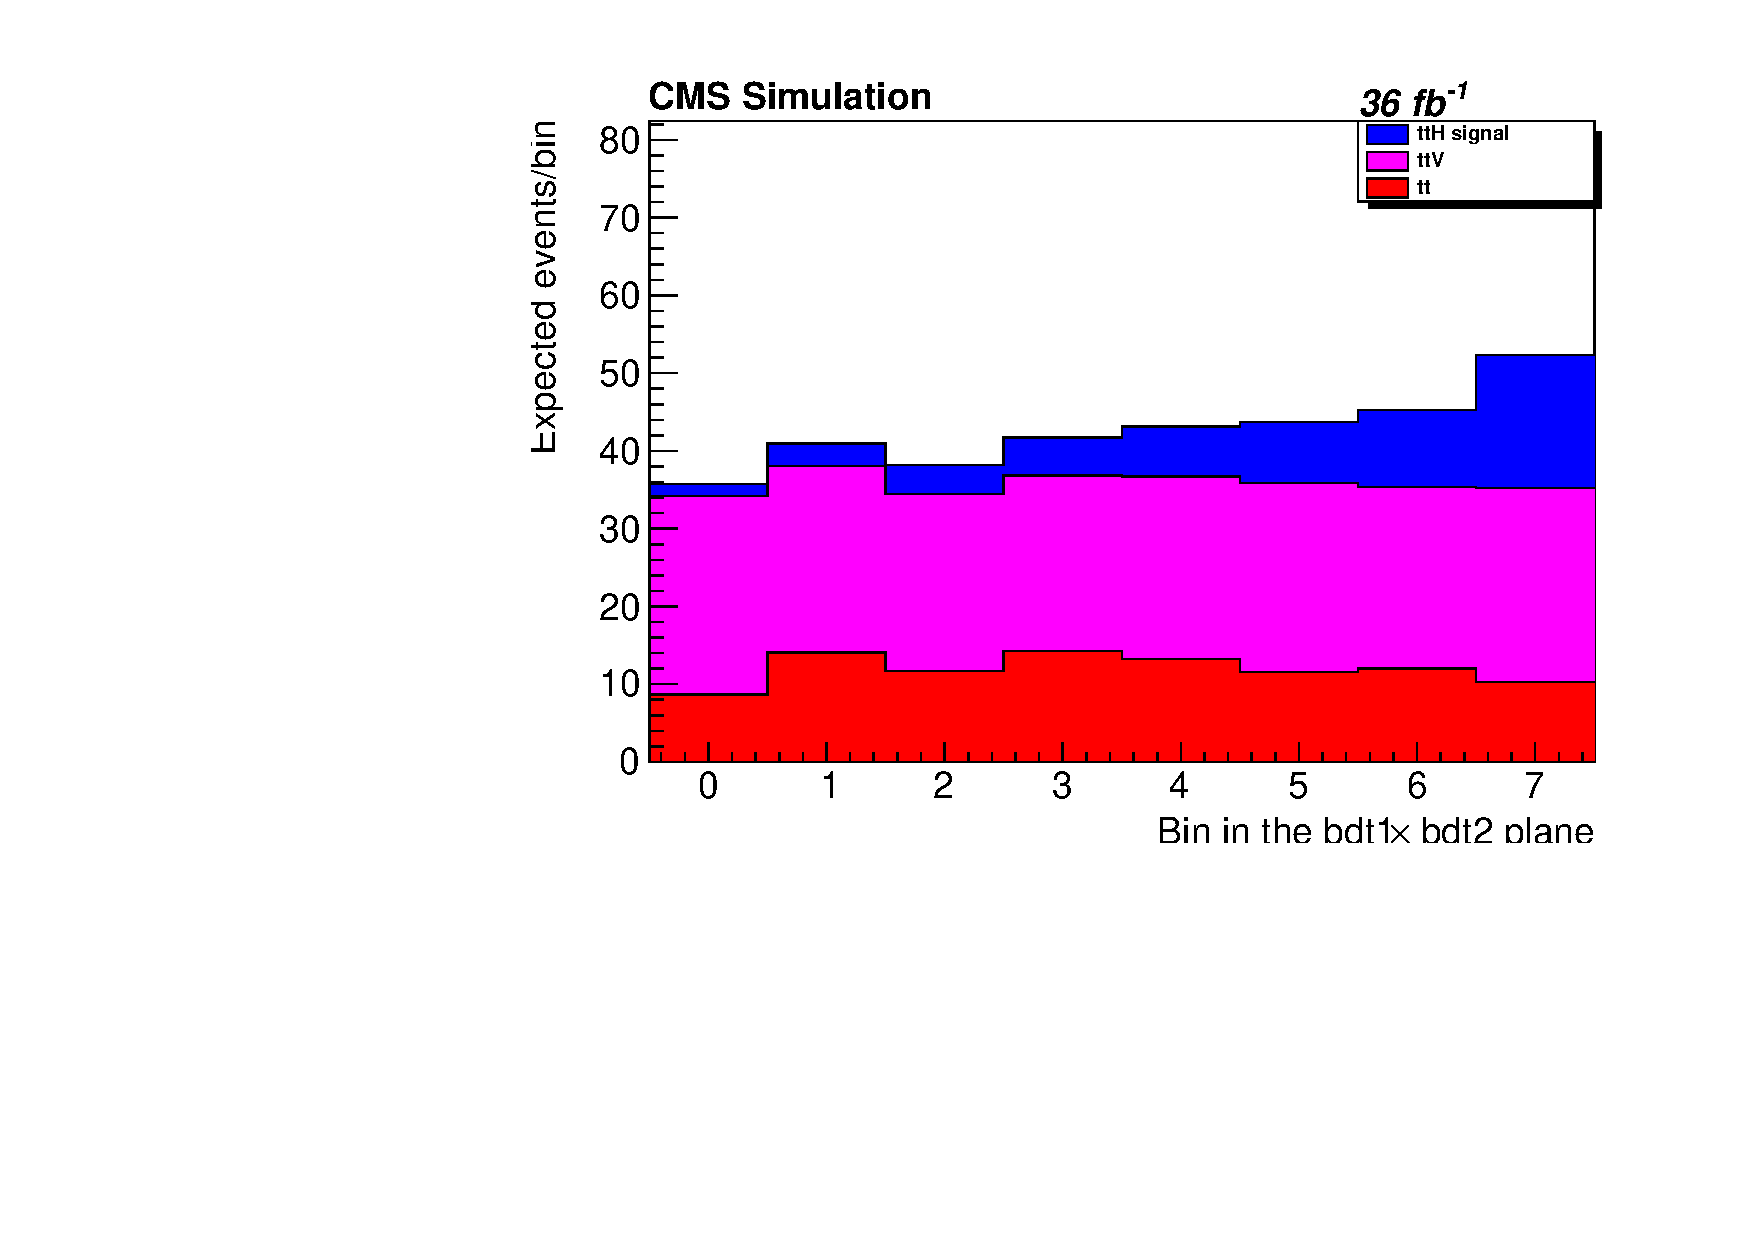
\includegraphics[width=0.49\textwidth]{ch9_figs/likelihoodBased_1d_2lss.pdf}
\caption[The 2D and 1D binning based on the cumulative likelihood distribution]{The 2D (left) and 1D (right) binning based on the cumulative likelihood distribution.}
\label{fig:likelihood}
\end{figure}

\begin{figure}[htp]
\centering
%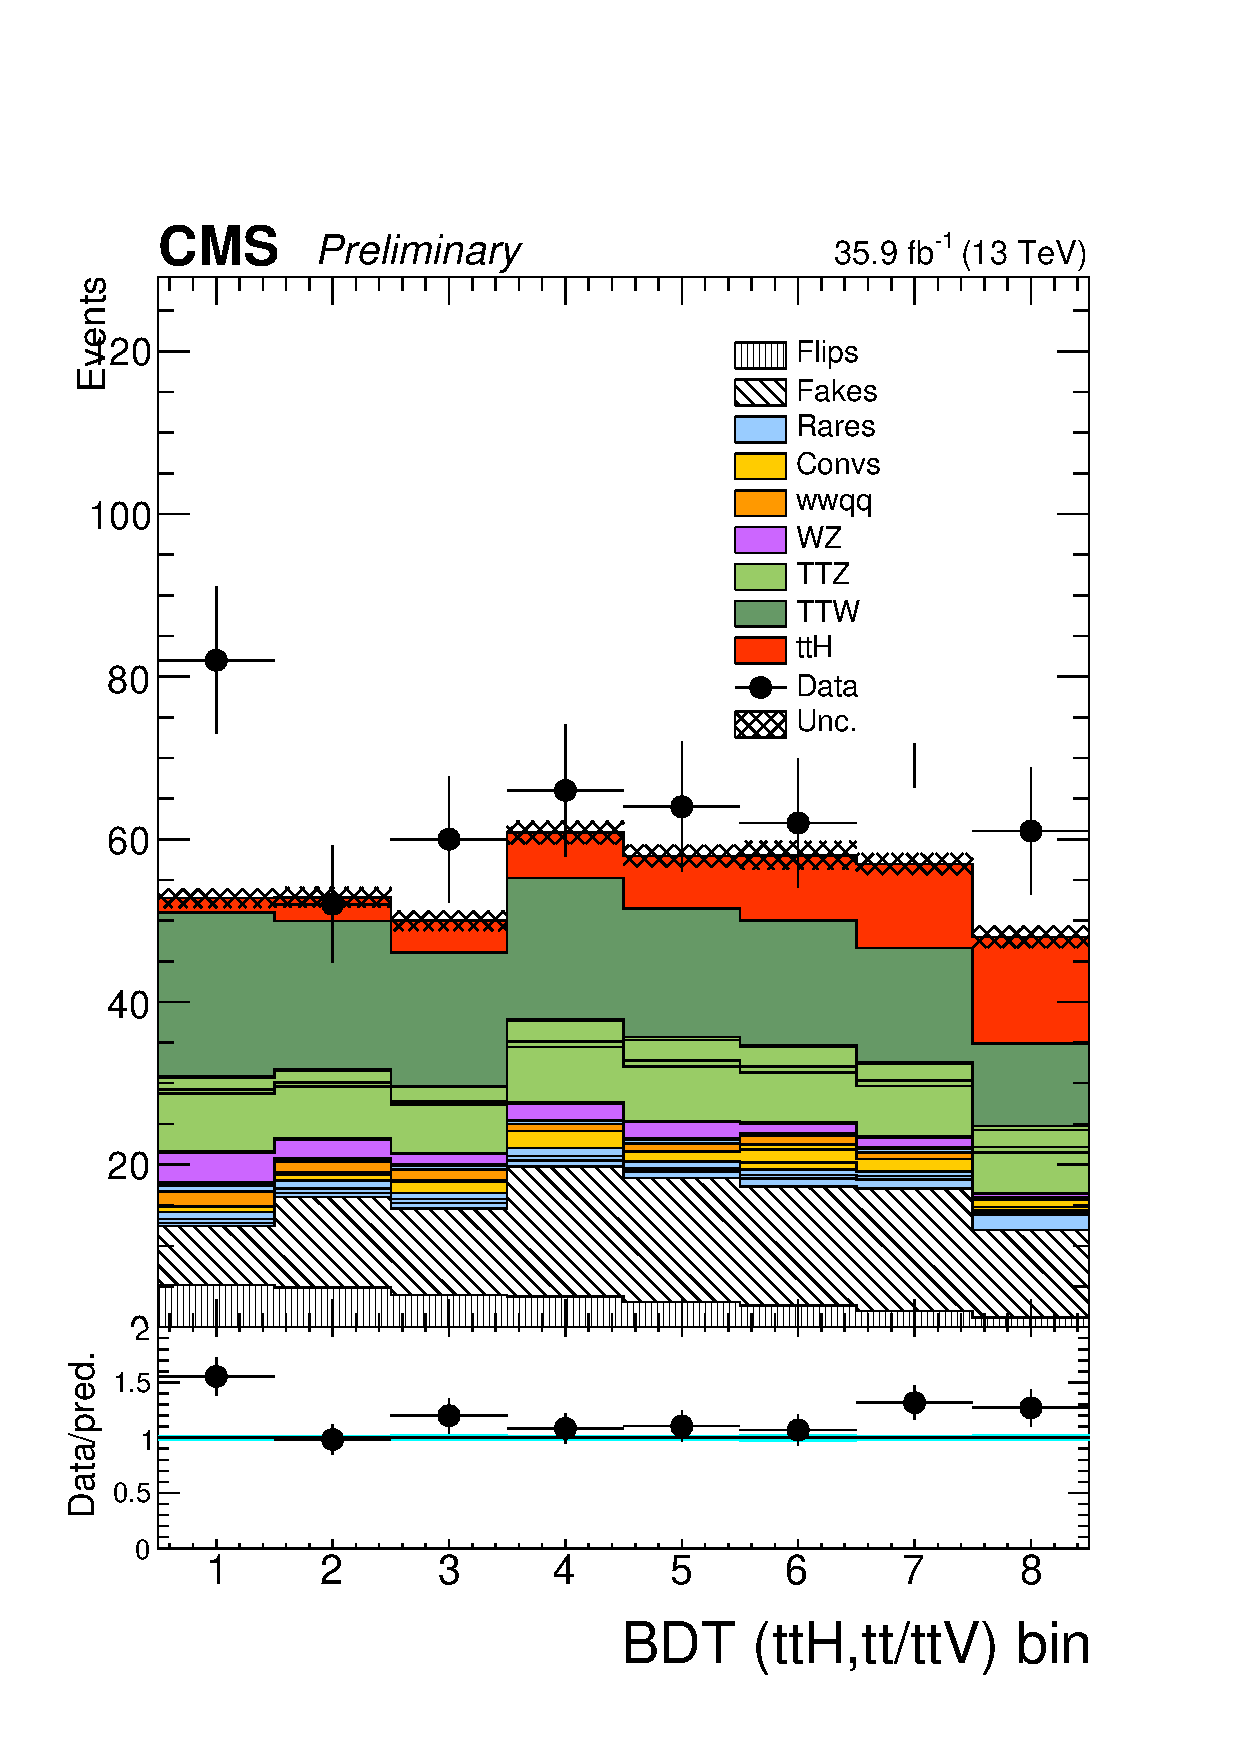
\includegraphics[width=0.49\textwidth]{ch9_figs/final_shape__ttH_stackPlot_SR.pdf}\\
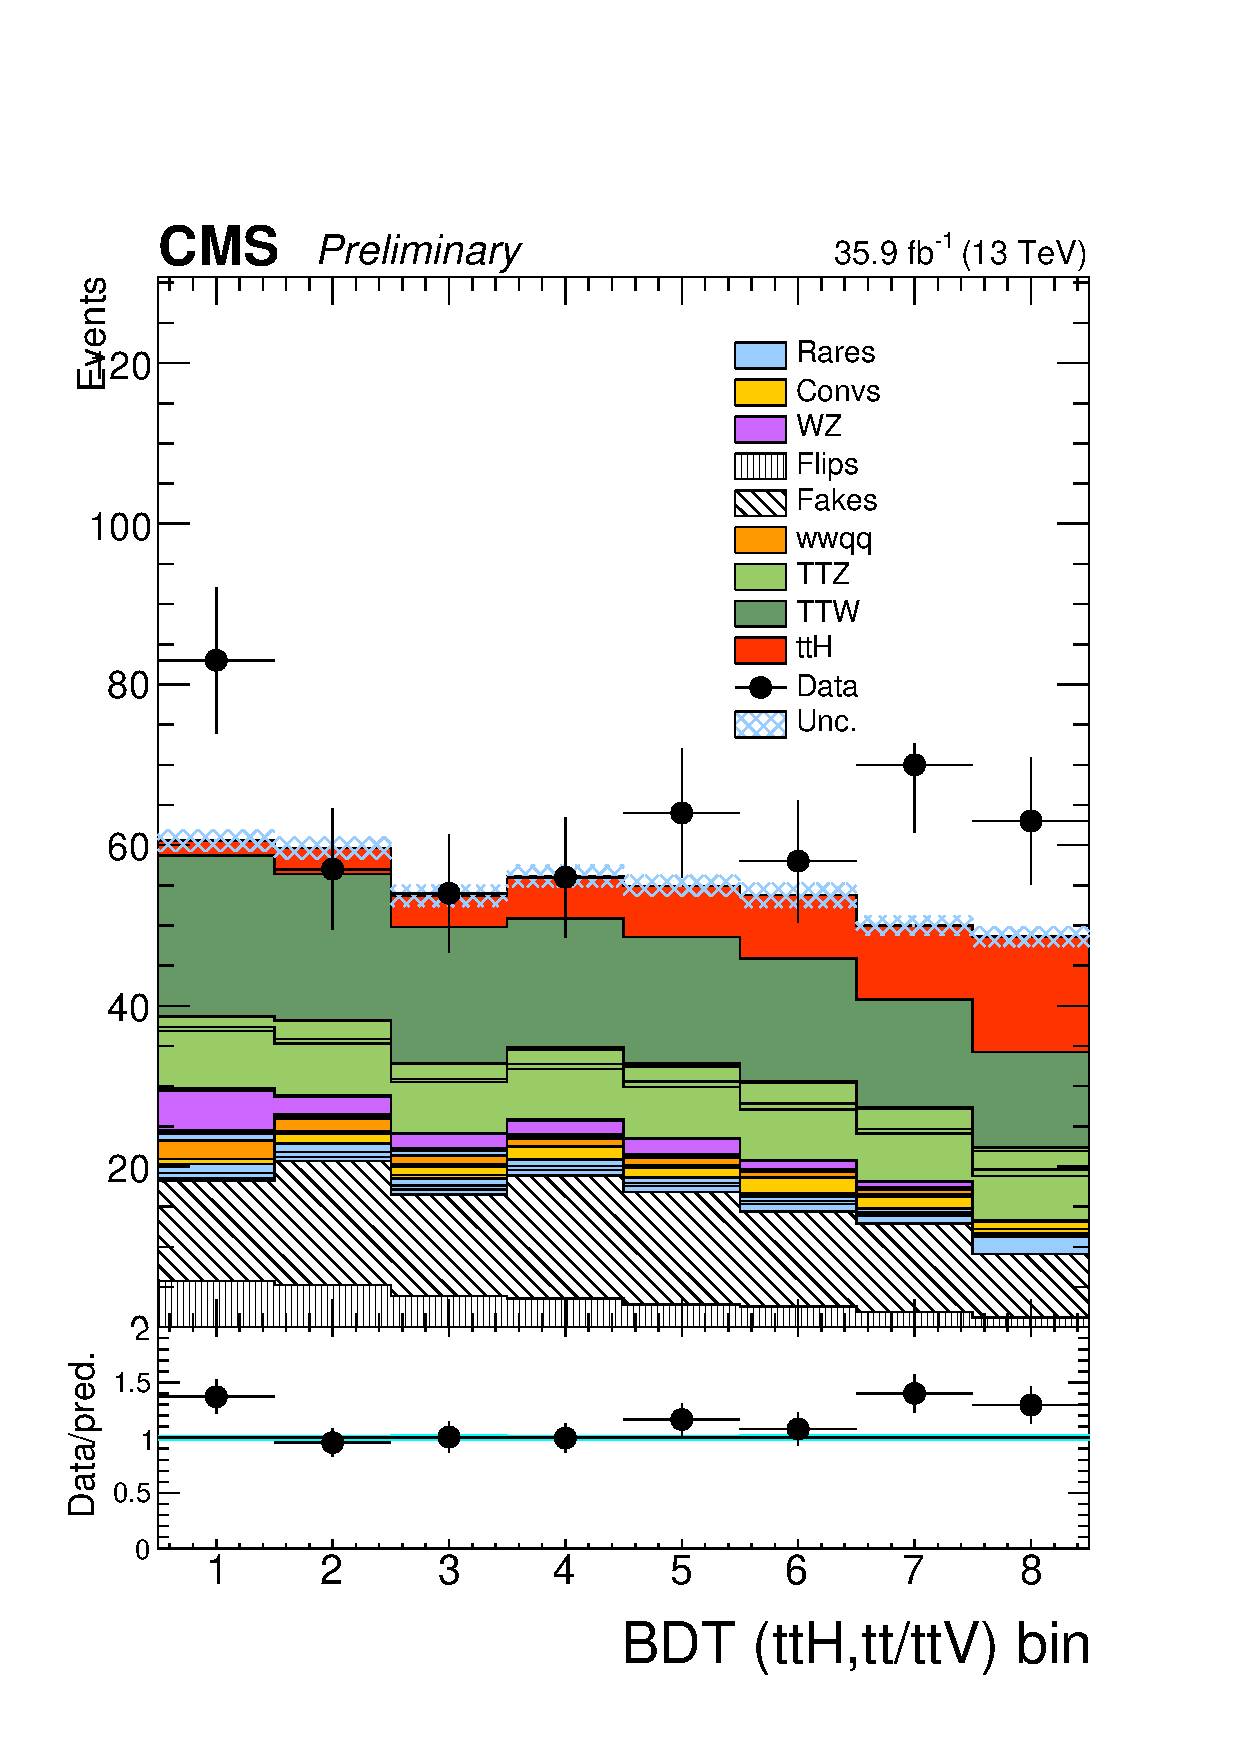
\includegraphics[width=0.49\textwidth]{ch9_figs/final_shape_bdtv8__ttH_stackPlot_SR.pdf}\\
%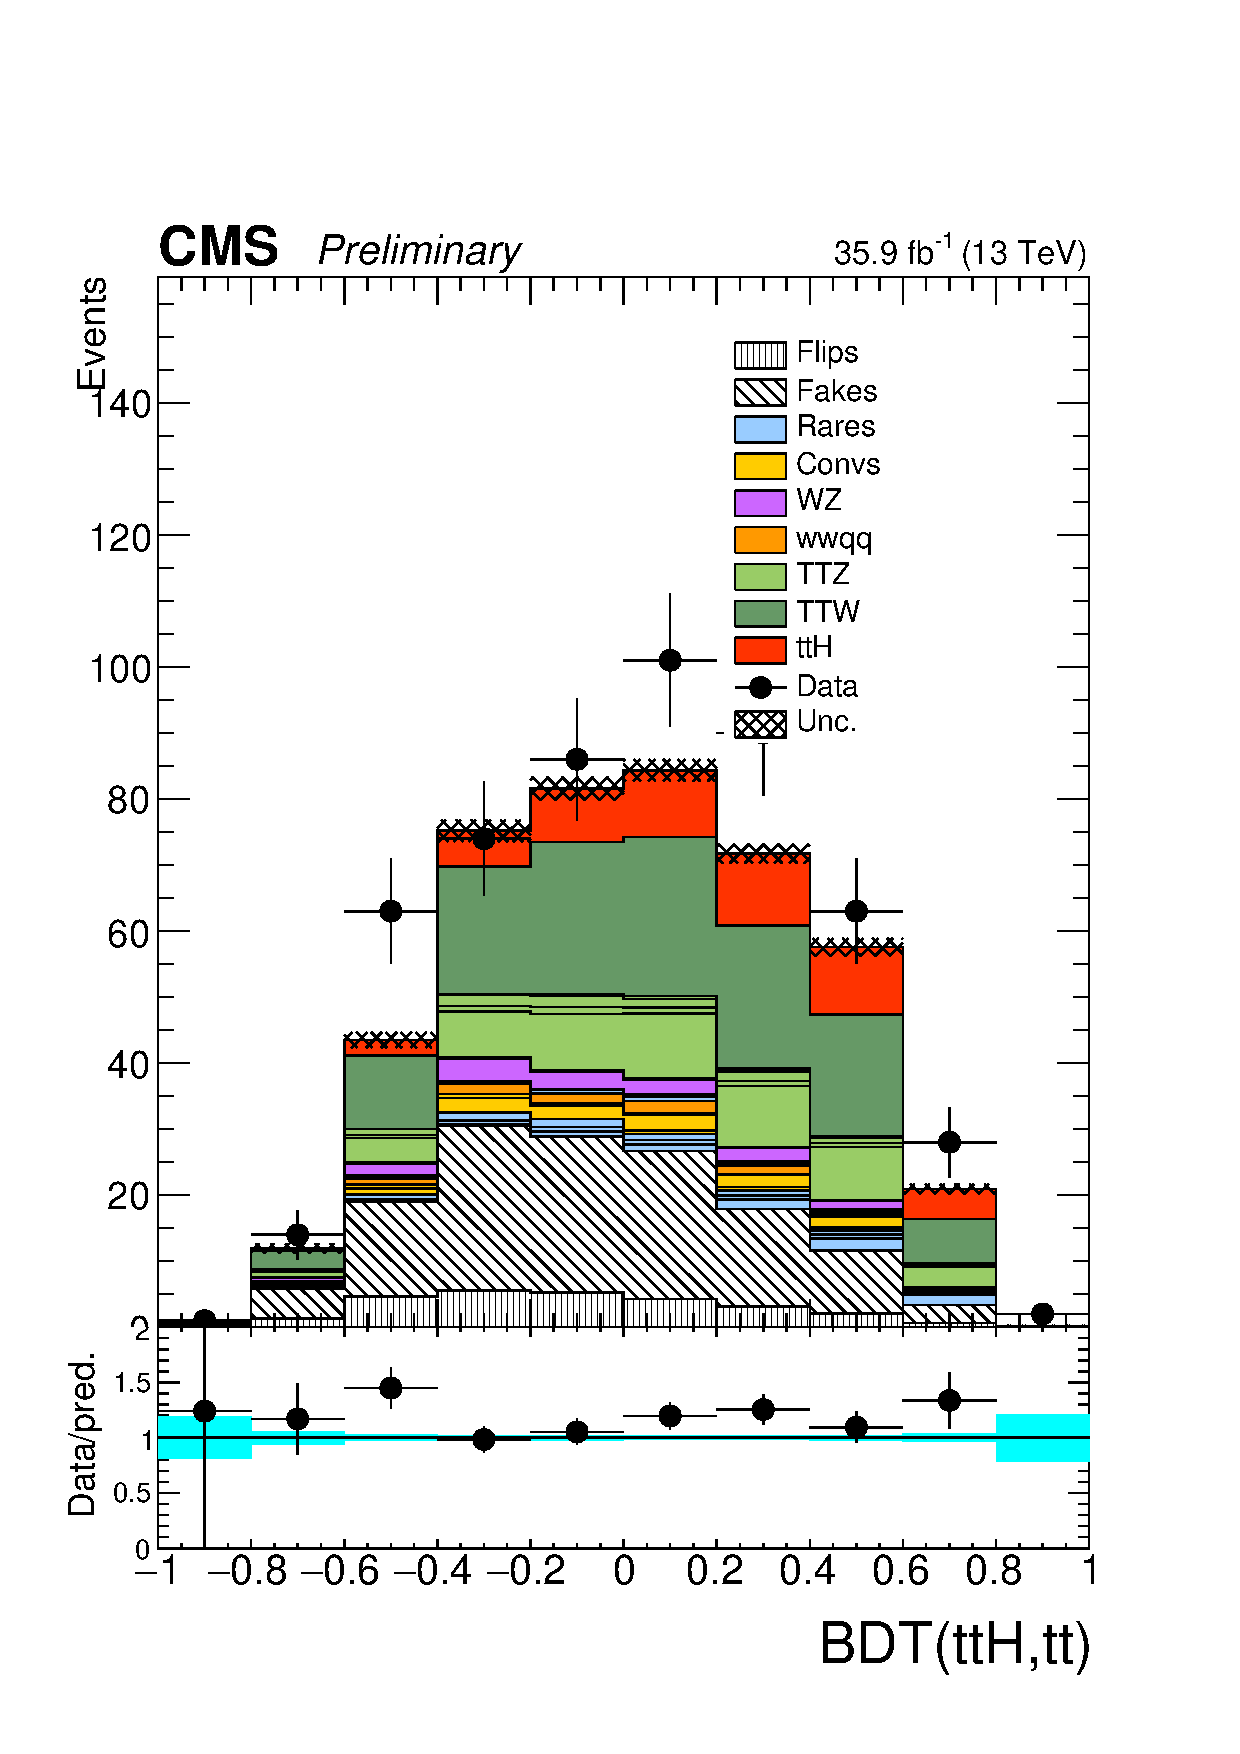
\includegraphics[width=0.49\textwidth]{ch9_figs/tt_BDT_ttH_stackPlot_SR.pdf}
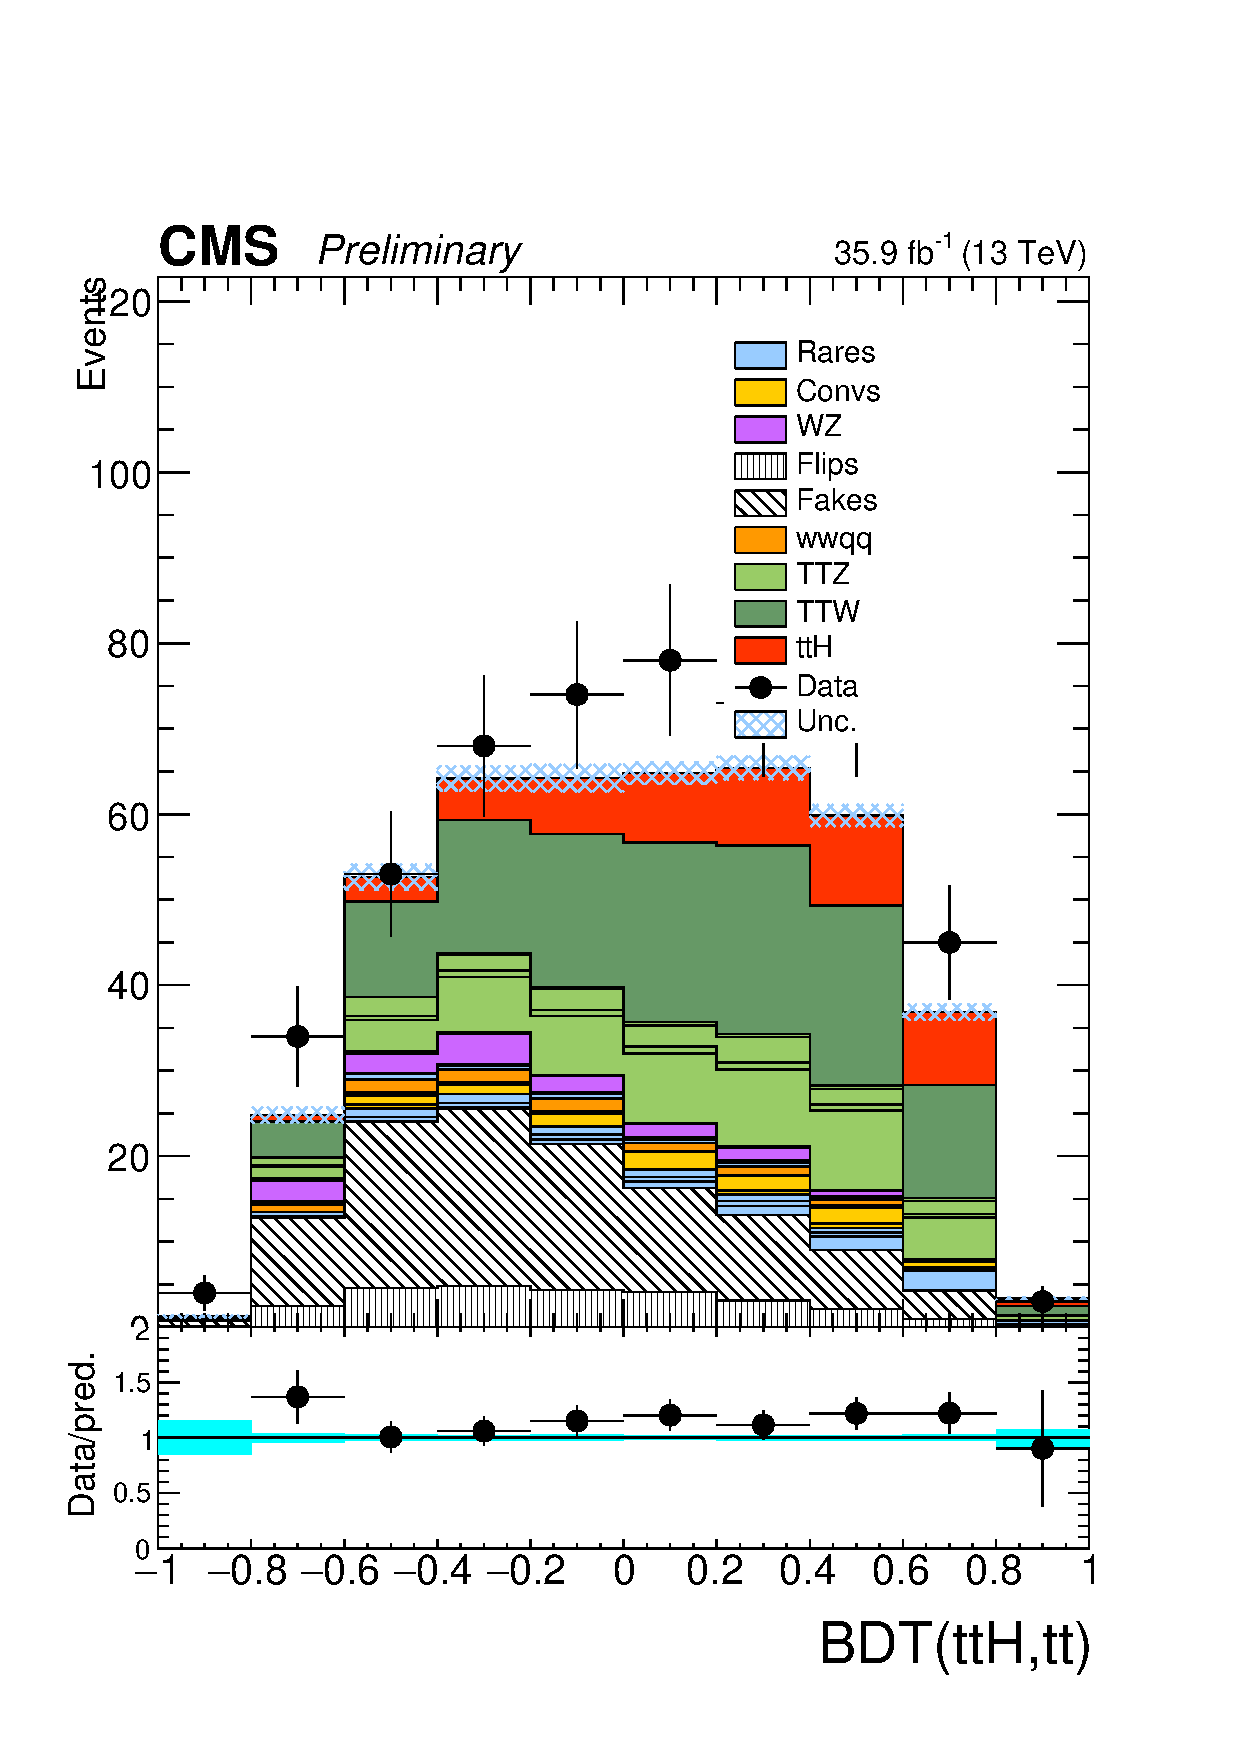
\includegraphics[width=0.49\textwidth]{ch9_figs/tt_BDT_BDTv8_ttH_stackPlot_SR.pdf}
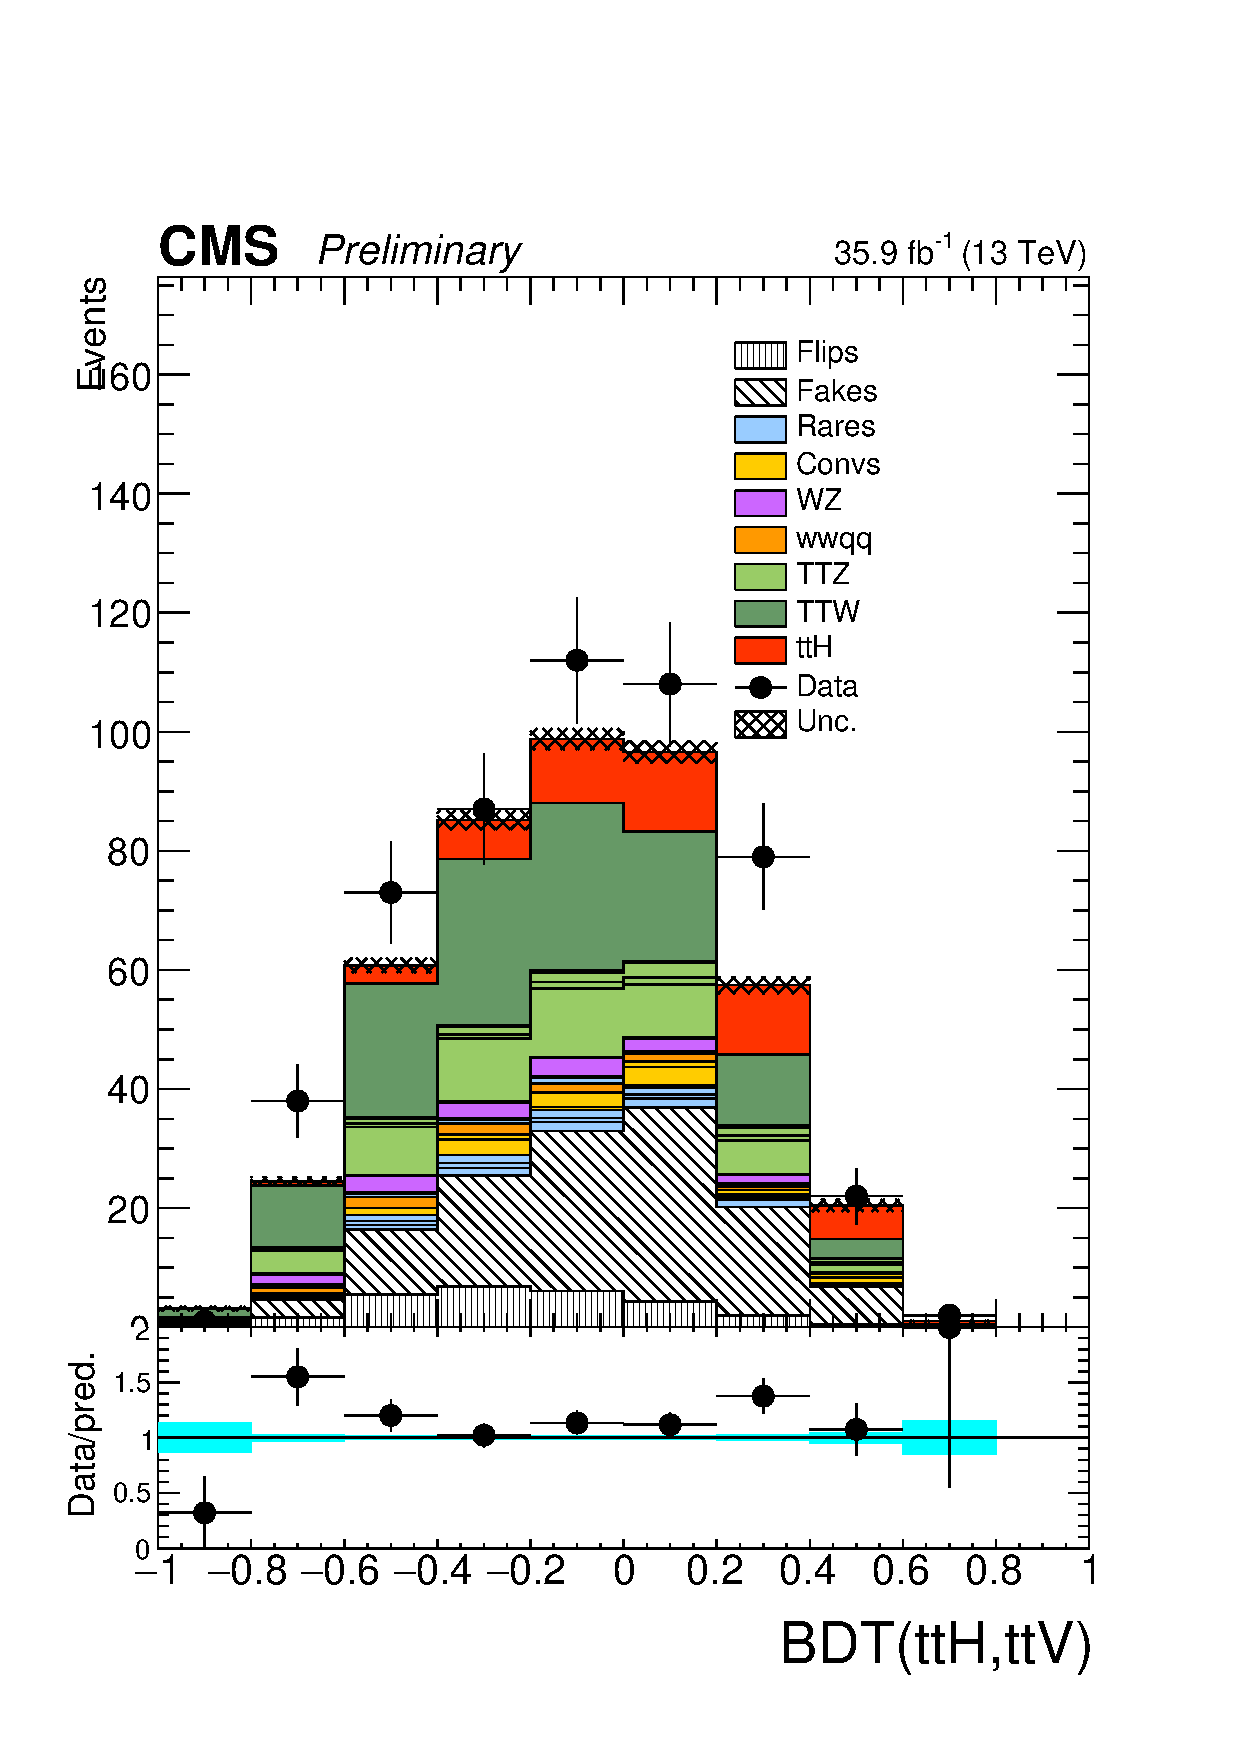
\includegraphics[width=0.49\textwidth]{ch9_figs/ttV_BDT_ttH_stackPlot_SR.pdf}
\caption[Data to MC comparison of final shapes]{The final 1D shape used for the analysis (top), the \ttbar BDT output (left) and the \ttv BDT output (right)}.
\label{fig:final_shapes_prefit}
\end{figure}


\section{Subcategorization}
In addition to the signal region categorization by lepton flavor, further categorization is applied to exploit differences between signal and background. All categories
split by the sum of the lepton electric charges. This splitting helps to isolate the \ttw background, which is asymmetric in lepton charge sum due to the initial state of the
diagram involving two incoming quarks. Because the LHC collides protons whose quark content is $uud$, this favors positively charged final states, while the \tth process
is initiated by gluon scattering, resulting in neutral final states, symmetric in lepton electric charge sum.
The signal region categories
are split further into two subcategories $b-tight$, which contains events with two b-jets passing the CSVv2 medium working point, and $b-loose$ which contains all other events
(those with fewer than 2 CSVv2 M jets). This splitting helps to separate \tth from the fake lepton background which is primarily comprised of \ttbar. Due to the same-sign 
lepton electric charge requirement, most of the \ttbar is vetoed, however there is a substantial amount of fakes originating from the b-decay. The b-jet is typically cleaned
from the fake lepton while the fake lepton is kept. This produces events with a single b-jet, while \tth should more often have two b-jets. In total there are 10 categories
making up the signal region, illustrated in Figure~\ref{fig:subcats} below. The $ee$ channel is not split according to b-jet content due to low statistics. 
It is the final shapes in these subcategories that are used for the final tabulation of signal, background, and data. 

\begin{figure}[htp]
\centering
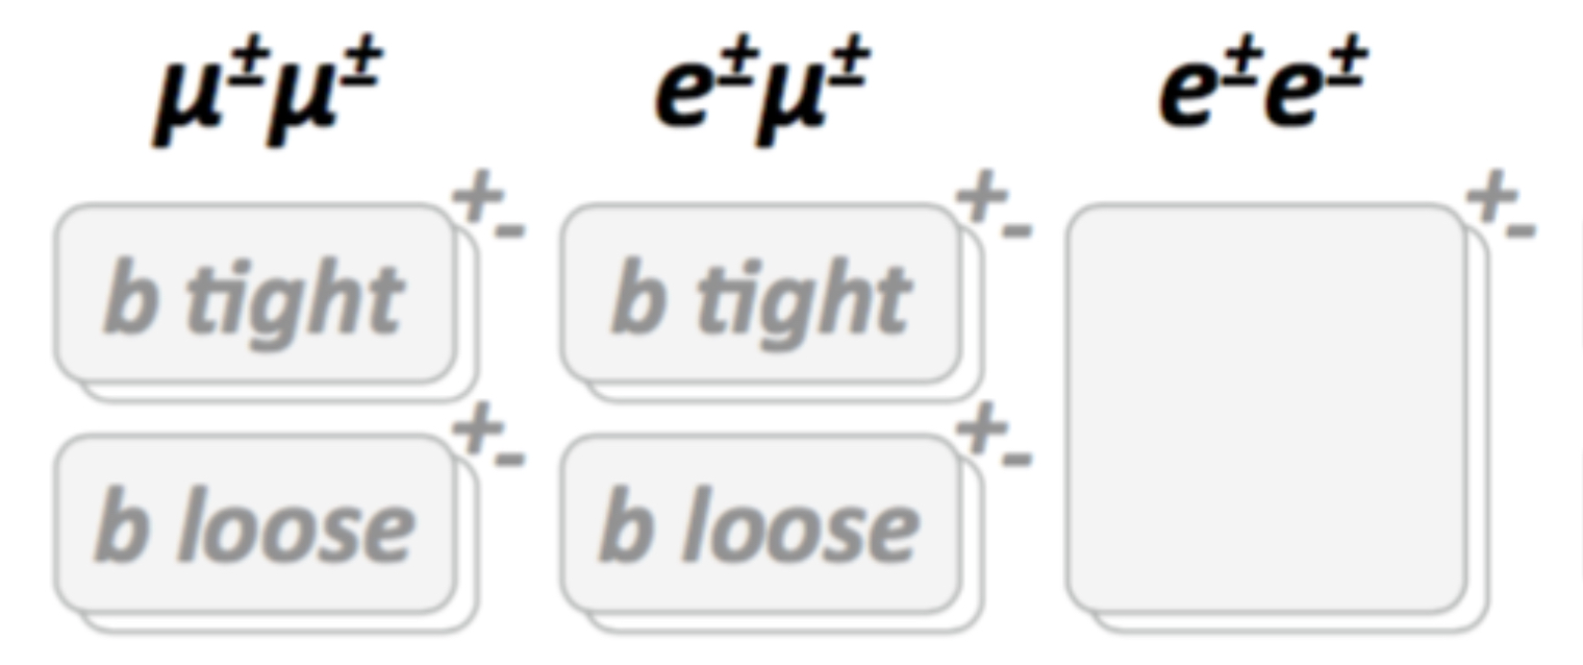
\includegraphics[width=0.7\textwidth]{ch9_figs/subcats.pdf}
\caption[Sub categories used for signal extraction]{The 10 subcategories used for signal extraction.}
\label{fig:subcats}
\end{figure}


